\chapter{The AIT QKD Stack}
\label{chap:The AIT QKD Stack}

The QKD Stack is the core component of QKD. Here the sifting, as in BB84, takes place, the keys are corrected via a classical channel, confirmed, analyzed, etc.

\medskip

The design of this stack is a series of separate processes which take their input from the previous process, process it and post the output to the next process, much like pipes in standard UNIX. Each of these processes exhibit a certain interface qualifying them to be a \emph{QKD Module}.

\medskip

A QKD Module \textbf{read}s a \emph{QKD Key} from the previous module via the \emph{pipe-in} interface point, \textbf{send}s and \textbf{recv}(receives) \emph{QKD Messages} with the same module on the peer side by utilizing the \emph{pipe-peer} at Alice's or \emph{pipe-listen} on Bob's side and finally \textbf{write}s the modified QKD Key as output into the \emph{pipe-out} sink.

\medskip

\begin{figure}[h]
    \centering
    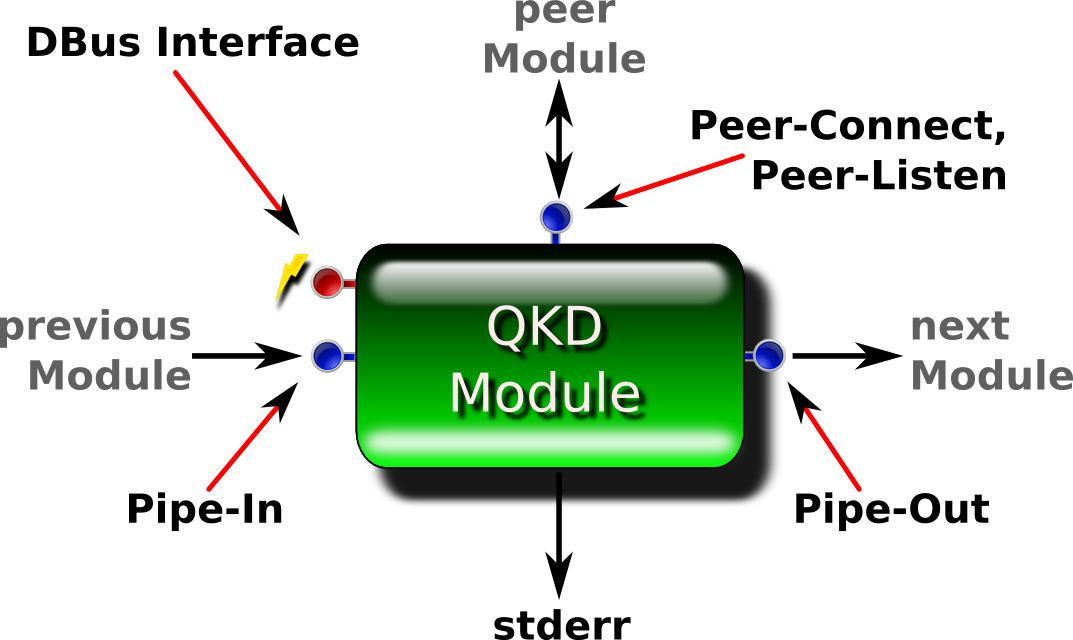
\includegraphics{./gfx/qkd-module.png}
    \caption{An AIT QKD Module.}
    \label{fig:qkd-module}
\end{figure}

The main functions \texttt{read}, \texttt{write}, \texttt{send} and \texttt{recv} are provided by the AIT QKD Framework. A QKD Key in the AIT QKD Framework is defined of all the bits and some header data holding meta information such as key identifier, error rate, number of disclosed keys, etc.

\medskip

Each QKD Module in the QKD pipeline serves a dedicated task, which it tries to fulfill in a best possible way. Among the QKD Modules deployed by AIT and accompanying the AIT QKD Framework include - but are not limited to:

\begin{itemize}

    \item BB84 sifting

    \item Error Correction

    \item Confirmation

    \item Privacy Amplification

\end{itemize}

In order to distinguish modules from one another every module does include an identifier like ``bb84''. However, more than one instance of a single QKD Module can be run in parallel on a system. By adding the process id of the operating system to the id uniquely names a QKD post process module within a QKD pipeline.

\medskip

As each QKD Module is segregated to work just on its dedicated task, it is fairly easy to modify or totally rewrite a single QKD Module without any impact for the rest of the modules in the pipeline.

\medskip

A QKD Module is usually started as a separate process. Any QKD Modules shipped with the R10 which has been created by the AIT QKD team does have this synopsis (example qkd-auth):

\begin{minipage}{0.9\textwidth}
\bigskip
\begin{verbatim}
$ qkd-auth --help
qkd-auth - AIT QKD Module 'Authentication' V0.10.1

This is an AIT QKD module.

This module provides authentication facilities to a QKD keystream.

Copyright 2012, 2013 AIT Austrian Institute of Technology GmbH

        Usage: bin/qkd-auth [OPTIONS]

Allowed Options:
  -b [ --bob ]          set this as bob's instance, the responder
  -c [ --config ] arg   configuration file URL
  -d [ --debug ]        enable debug output on stderr
  -h [ --help ]         this page
  -r [ --run ]          run immediately
  -v [ --version ]      print version string
\end{verbatim}
\medskip
\end{minipage}

The options are:

\begin{itemize}

\item{\textbf{\texttt{--bob}}}: If set starts the QKD Modules with the role of \emph{Bob} assigned. If this option is omitted the module's role is set to \emph{Alice}.

\item{\textbf{\texttt{--config arg}}}: This reads in a configuration file specified by \texttt{arg}.

\item{\textbf{\texttt{--debug}}}: This immediately turns debug output on and creates output on \texttt{stderr}.

\item{\textbf{\texttt{--help}}}: A small summary of available options of and arguments to the module.

\item{\textbf{\texttt{--run}}}: When this option is given, the module switches immediately to the \emph{RUNNING} state and starts key processing. If not the module switches into the \emph{READY} state and awaits the "\texttt{run()}" method call. \\ \\
Hint: we recommend using this option only along the \texttt{--config} option since without it the module will run its default setup configuration with no pipe-in/out set up.

\item{\textbf{\texttt{--version}}}: Give a version information about the current module implementation.

\end{itemize}

\clearpage

\noindent Example:

\begin{minipage}{0.9\textwidth}
\bigskip
\begin{verbatim}
$ qkd-confirnation
\end{verbatim}
\medskip
\end{minipage}

This starts the qkd-confirmation module. The module is launched as \emph{Alice} and its configuration is set to default values. The module has already connected the DBus and publishes values and methods on the bus.

\medskip

However, the module is not connected to nowhere: it is dangling loose within the system, no module before, none after. To connect this module and integrate it into QKD pipeline, the user has to set the pipe-in/out connection points accordingly and call the \texttt{run()} DBus command.

\medskip

\noindent Example:

\begin{minipage}{0.9\textwidth}
\bigskip
\begin{verbatim}
$ qkd-bb84 --bob --config /etc/qkd/bb84.config --run
\end{verbatim}
\medskip
\end{minipage}

This example is quite different: the module starts and picks its setting from the configuration file located at \texttt{/etc/qkd/bb84.config}. Within this configuration file hopefully the pipe-in/out addresses are set (and much more, see section \ref{subsec:Module Configuration}).

\medskip

Picking the right configuration settings depends also on the current module's role setting. That is why the \texttt{--bob} switch sets this QKD Module process instantly to act as \emph{Bob}.

\medskip

Last but not least is the module told to immediately get into processing keys. The \texttt{--run} switch will instantly start key processing by requesting keys from the previous module -- if the module's configuration successfully set an address.


\section{Anatomy of a QKD Module}
\label{sec:Anatomy of a QKD Module}

An AIT QKD Module is realized as a single UNIX process. But despite common characteristics of such operating system processes an AIT QKD Module has way more interfaces to interact with its environment.

\begin{table}[h]
    \begin{tabular}{lp{11.5cm}}
    Name            &   Description \\
    \hline
    \\
    Pipe-In         &   This is the interface where keys from previous modules are accepted. This is the input channel of the module's key reconciliation work.\\ [0.7em]
    Pipe-Out        &   Once the module has done working on the key this is the place to push the key to. Here the next module awaits the data.\\ [0.7em]
    Peer-Connect    &   This is the interface at which \textbf{Alice} sends and receives key reconciliation data to and from Bob.\\ [0.7em]
    Peer-Listen     &   \textbf{Bob} creates a listen interface to wait for Alice to connect. Once Alice connected, Bob and Alice exchange key data in order to process on the current key.\\ [0.7em]
    DBus Interface  &   Every AIT QKD Modules offers some properties and methods exposed to the environment. Among these are e.g. current module state, aggregated bits process so far and terminating the module gracefully.\\ [0.7em]
    stderr          &   Finally debug messages can be printed on \texttt{stderr} if enabled.\\ [0.7em]    
    \end{tabular}
    \caption{QKD Module interfaces}
    \label{tab:QKD Module interfaces}
\end{table}

\medskip

Table \ref{tab:QKD Module interfaces} summarizes the main interfaces of an AIT QKD Module. Most import are the pipe-in and the pipe-out interface points. They are more elaborated in section \ref{subsec:Reading and Writing QKD keys}. Roles are also very essentials to a QKD Module, see section \ref{subsec:Module Roles}. Every AIT QKD Module already offers a catalog of properties and functions via DBus to manage the module.

\medskip

Special note for the debug output on \texttt{stderr}: every AIT QKD Module (and also the Q3P node) do have a property \texttt{debug} which is accessible via DBus. It turns the debug output on or off. Debug output is always pushed to the UNIX standard \texttt{stderr} stream. In order to distinguish the output from one module to another we highly recommended to start every module with a redirected \texttt{stderr} output already even though \texttt{debug} might not be enabled.

\begin{minipage}{0.9\textwidth}
\bigskip
\begin{verbatim}
$ my-qkd-module 2> my-qkd-module.debug
\end{verbatim}
\medskip
\end{minipage}

Shown above is a command line of a fictive AIT QKD Module ``my-qkd-module'' with its \texttt{stderr}-output redirected to a file called "my-qkd-module.debug". This is useful since any time you encounter problems you may turn on this \texttt{debug} flag at will and this will produce valid debug information.

\medskip

Beware: debug output generation does consume some CPU power. Even worse: sometimes the debug output has to be pretty formated and prepared which increases costs of key reconciliation drastically. Do not set this flag to "on" when you do not intend to use the generated output.

\medskip

Besides the debug flag also syslog\footnote{http://en.wikipedia.org/wiki/Syslog} will be fed by the AIT QKD Modules. These syslog messages are rare in comparison to debug messages. They are of informative, warning or critical nature. Opposed to the debug messages you can not turn of syslog messages creation.    

\subsection{Module Threads}
\label{subsec:Module Threads}

An AIT QKD Module is created as a multi-threaded process. This is intentionally to keep up the AIT QKD Module responsive at almost any stage or state it is in.

\medskip

There are at least three threads running:

\begin{enumerate}

\item{Main Thread}: this is the thread initially started by the operating system. This one starts up all QKD Module subsystems, launches all other threads and waits until the QKD Modules ceased.

\item{QKD Thread}: the QKD thread does the real QKD post processing work. This does the sifting, error correction, confirmation, privacy amplification, ... you name it!

\item{DBus Thread}: while the main thread orchestrates every aspect of the module and the QKD thread works on keys, this DBus thread listens on the DBus to take queries, look up property values and return them back to the bus. Also this thread is active when a certain method of the AIT QKD Module has been invoked "from the outside".

\end{enumerate}

The advantage of having a multi-threaded QKD application running is the segregation of management and work right inside the module itself. Plus creation of additional "worker" threads to possibly exploit some parallel characteristics of certain QKD algorithms. This is already laid out, since all concurrent data access and execution paths should be safe inside the AIT QKD Module.

\medskip

But multi threading is a daunting business and can lead to quite complex situations. AIT QKD programmers are free to use any multi threading paradigm of choice. This is great power. Accompanied with great responsibility.

\medskip

In the ``Running'' state (see next section \ref{subsec:Module States}) the QKD Module worker mainly runs the internal \texttt{process()} function. This functions is run after a key has been PULL'ed from the previous module and before it is PUSH'ed to the next.

\medskip

If debug output is enabled then this is seen as (line breaks inserted for the ease of reading, key-PULL and key-PUSH are placed on one single line):

\begin{minipage}{0.9\textwidth}
\bigskip
\begin{verbatim}
key-PULL [000000000005036ms] 
                        id: 0000000058 bits: 0000009976 
                        err: 0000000032 dis: 0000000513 crc: 75436080 
                        state: corrected
confirmation for key 58 ok
key-PUSH [000000000005088ms] id: 0000000058 bits: 0000009976 
                        err: 0000000032 dis: 0000000513 crc: 75436080 
                        state: confirmed
                        dur: 000051891000 ns (000052 ms)
\end{verbatim}
\medskip
\end{minipage}

This sample above is taken from the confirmation module as the QKD worker thread for this specific module adds the "confirmation for key 58 ok" into the output. The lines starting with "key-PULL" and "key-PUSH" are always present by \emph{every} module in debug mode turned on.

\medskip

Table \ref{tab:QKD Module key-PULL and key-PUSH} explains the field given in those lines.

\begin{table}[h]
    \begin{tabular}{lp{7.5cm}}
    Field                   &   Description \\
    \hline
    \\
    key-PULL                &   This line describes the reception of a key from the previous module.\\ [0.7em]    
    key-PUSH                &   This line describes the forwarding of a key to the next module.\\ [0.7em]    
    [000000000005088ms]     &   Timestamp of action in milliseconds.\\[0.7em]
    id: 0000000058          &   Key Id.\\[0.7em]
    bits: 0000009976        &   Bits read/written. This is the size of the key.\\[0.7em]
    err: 0000000032         &   Error Bits corrected within the current key.\\[0.7em]
    dis: 0000000513         &   Number of disclosed bits of the current key leaked to the public.\\[0.7em]
    crc: 75436080           &   CRC-32 checksum in hexadecimal of the key.\\[0.7em]
    state: corrected        &   Current state of the key.\\[0.7em]
    dur: 000051891000 ns (000052 ms)    &   Processing time used for this particular key in nanoseconds and milliseconds.\\[0.7em]
    \end{tabular}
    \caption{QKD Module key-PULL and key-PUSH values}
    \label{tab:QKD Module key-PULL and key-PUSH}
\end{table}

\medskip

\subsection{Module States}
\label{subsec:Module States}

The life cycle of an AIT QKD Module is covered by the AIT QKD Module states as shown in figure \ref{fig:qkd-module-states}.

\begin{figure}[h]
    \centering
    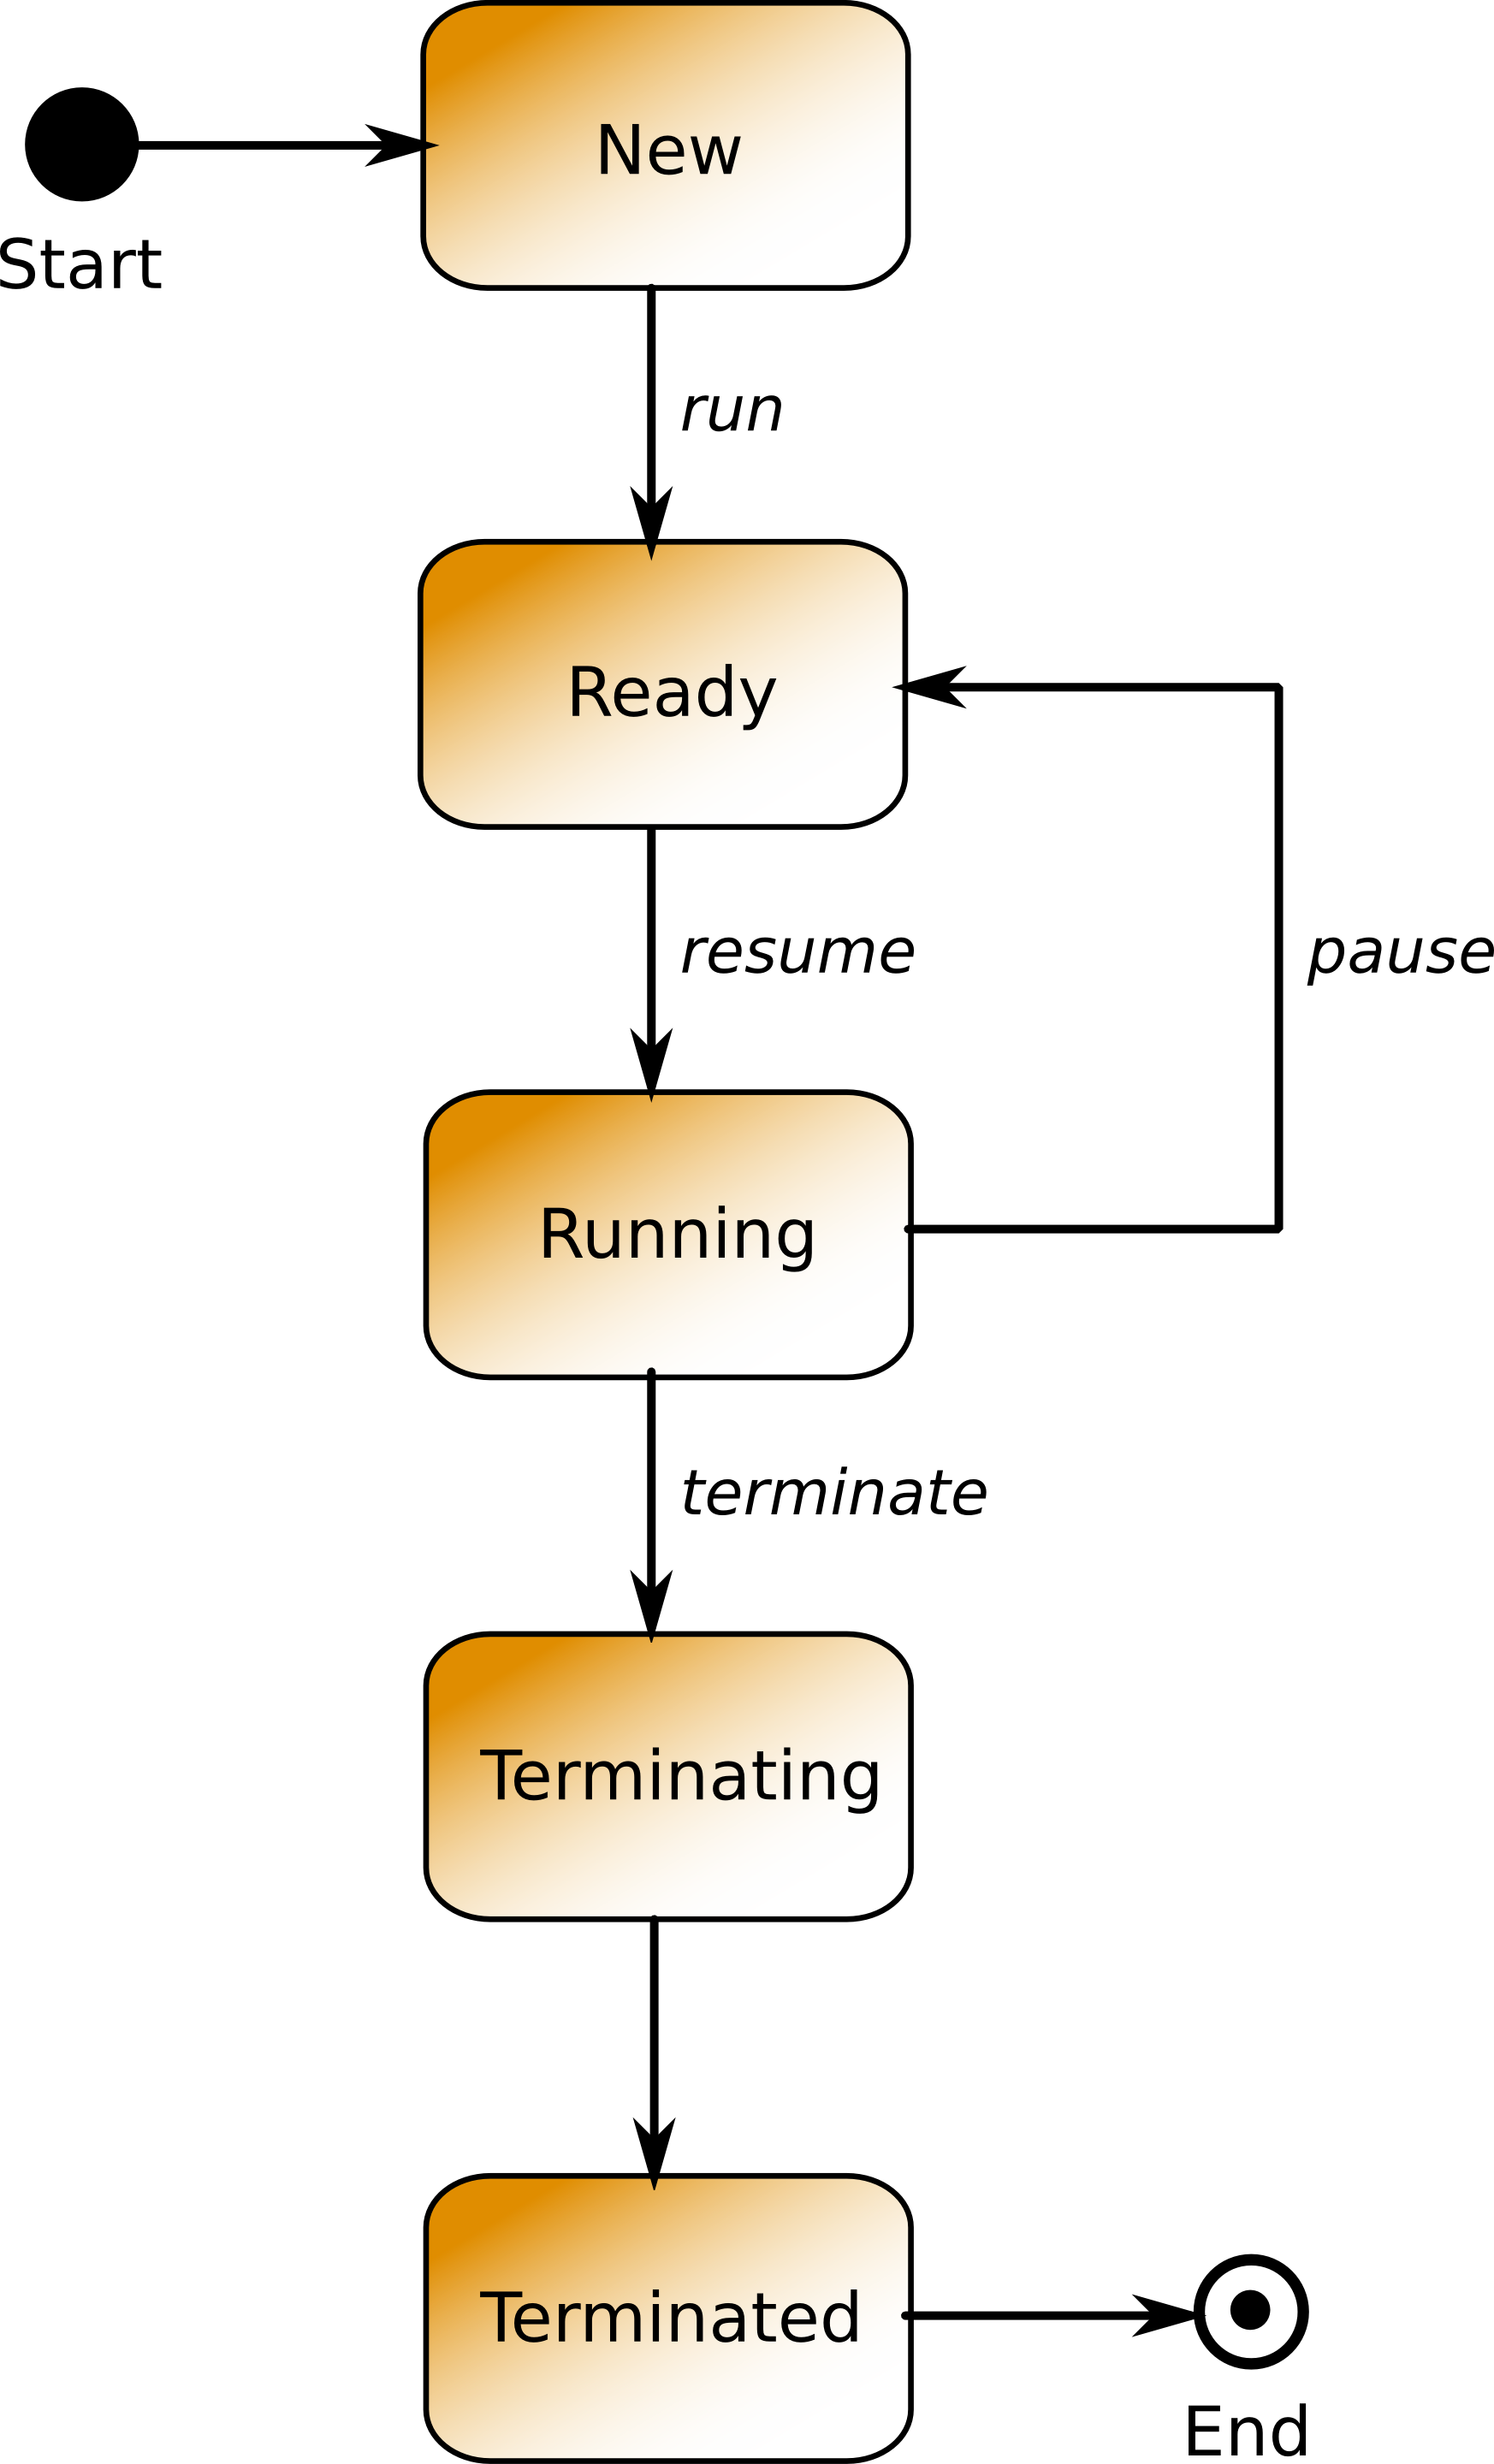
\includegraphics[scale=0.70,keepaspectratio=true]{./gfx/qkd-module-states.png}
    \caption{AIT QKD Module States.}
    \label{fig:qkd-module-states}
\end{figure}

\medskip

The states are:

\begin{itemize}

\item{\textbf{New}}: This is the initial state when the QKD Module object has been created an most values are set to default. In this state the module already registered to the DBus but no dedicated QKD Module worker thread has been spawned. \\[1em]
Also the Pipe-In/Out addresses are still left blank. Setting them is crucial for 
setting up a QKD pipeline.

\item{\textbf{Ready}}: This one is reached whenever the DBus method \texttt{run()} has been invoked. This initializes the QKD Module worker thread which is now eager to receive keys from the previous QKD Module. However at the current stage this thread is still hold back though all QKD relevant subsystems are up and running. The DBus method \texttt{resume()} switches the module to the next state.

\item{\textbf{Running}}: The QKD Module thread is pulling keys from the previous module, processing them and pushing the processed keys to the next module in the pipeline. On the DBus you can always call \texttt{pause()} to let the QKD worker thread pause current execution.

\item{\textbf{Terminating}}: Once the module received the \texttt{terminate()} command it switches into this state and winds down QKD subsystems.

\item{\textbf{Terminated}}: Here all QKD subsystems ceased and the QKD Module worker thread ended.

\item{\textbf{End}}: The QKD Module worker thread has been joined by the application's main thread. The program terminates finally.

\end{itemize}


\subsection{Module Roles}
\label{subsec:Module Roles}

Within the AIT QKD framework each module \textbf{must} have a role assigned before switching into the Ready state. The roles are either \emph{Alice} or \emph{Bob}. As the configuration parsing depends on whether the module is set to Alice or Bob this is a very essential trait.

\begin{itemize}

\item{\textbf{Alice}}: A module given the role as Alice will actively initialize communication. Picturing the classic client-server model, such QKD Modules act as client. All Alice QKD Modules will utilize the \texttt{pipe\_connect} interface to contact the peer remote. This is done actively.

\item{\textbf{Bob}}: A Bob module acts as server in the classic client-server paradigm. These modules will set up their \texttt{pipe\_listen} address and will wait for an Alice QKD Module to connect.

\end{itemize}

\begin{figure}[h]
    \centering
    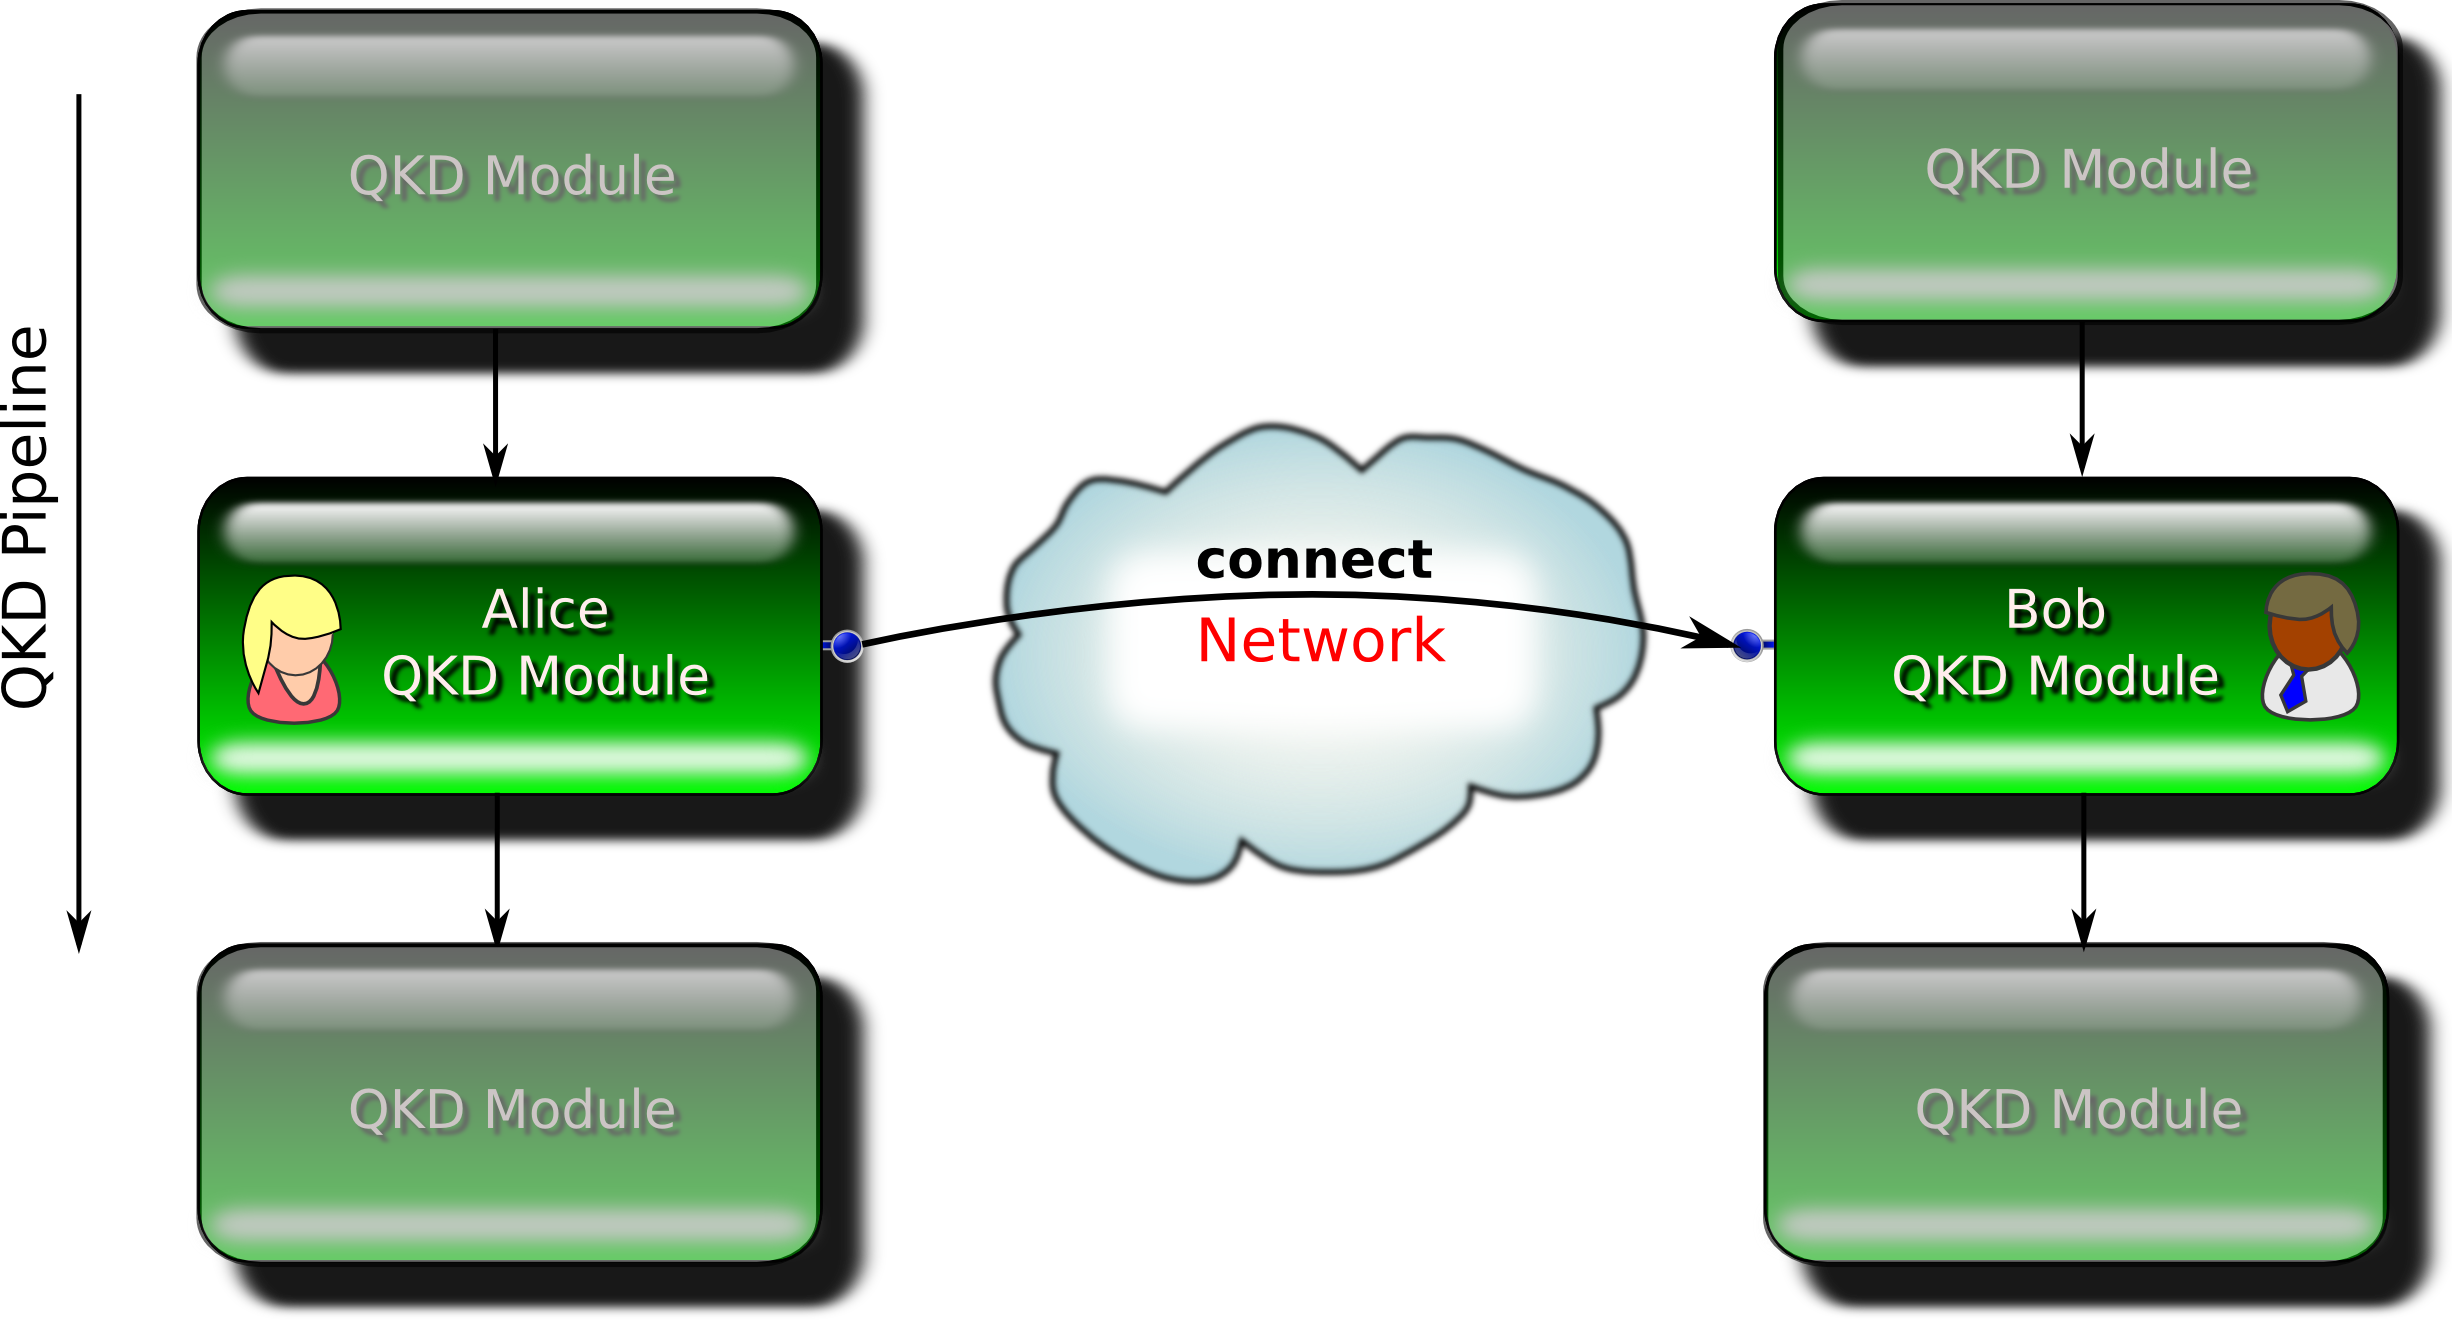
\includegraphics[scale=0.50,keepaspectratio=true]{./gfx/qkd-module-roles.png}
    \caption{AIT QKD Module Roles.}
    \label{fig:qkd-module-roles}
\end{figure}

\medskip

As in figure \ref{fig:qkd-module-roles}: always Alice connects to Bob. Alice plays the \emph{initiator} of protocol stages and Bob the \emph{responder}.

\medskip

But the role assignment of a pair of modules does not imply that all modules on one side are ought to have the same role. Quite contrary: no module is forced to respect the previous or next module's role and therefore Alice and Bob modules can be mingled in a single QKD pipeline on one side.

\medskip

Furthermore there are some QKD Modules which do not have a paired counterpart. If not stated otherwise these modules are assigned to act as Alice modules and read their configuration accordingly from the configuration files (see section \ref{subsec:Module Configuration}).

\medskip

When a module does expect a peer module, then it is called "paired". The "paired" state is present even if the module itself is not connected (yet) to the remote peer module.

\subsection{Reading and Writing QKD keys}
\label{subsec:Reading and Writing QKD keys}

As already mentioned above all QKD Modules do read their input keys from the previous modules and write their processed keys to the next. The address to pull keys from is \texttt{pipe\_in} and the address to push keys to is labeled  \texttt{pipe\_out}.

\medskip

As a rule for a QKD pipeline the input \texttt{pipe\_in} of a QKD Module \textbf{must} be the \texttt{pipe\_out} of the previous module. This is how a QKD pipeline is built up.

\vspace{2cm}

\begin{center}
\begin{minipage}{10cm}
\shadowbox{
\begin{minipage}{9cm}
Creating an AIT QKD pipeline is \textbf{only} achieved by setting one module's output address \texttt{pipe\_out} equal to the next module's input address \texttt{pipe\_out}.
\\[1em]
There is no other way.
\end{minipage}
}
\end{minipage}    
\end{center}

\vspace{2cm}

\clearpage

There are several places where you specify the module's \texttt{pipe\_in} and \texttt{pipe\_out} addresses. The main way how to do this is via configuration files, see section \ref{subsec:Module Configuration}.

\medskip

\begin{figure}[h]
    \centering
    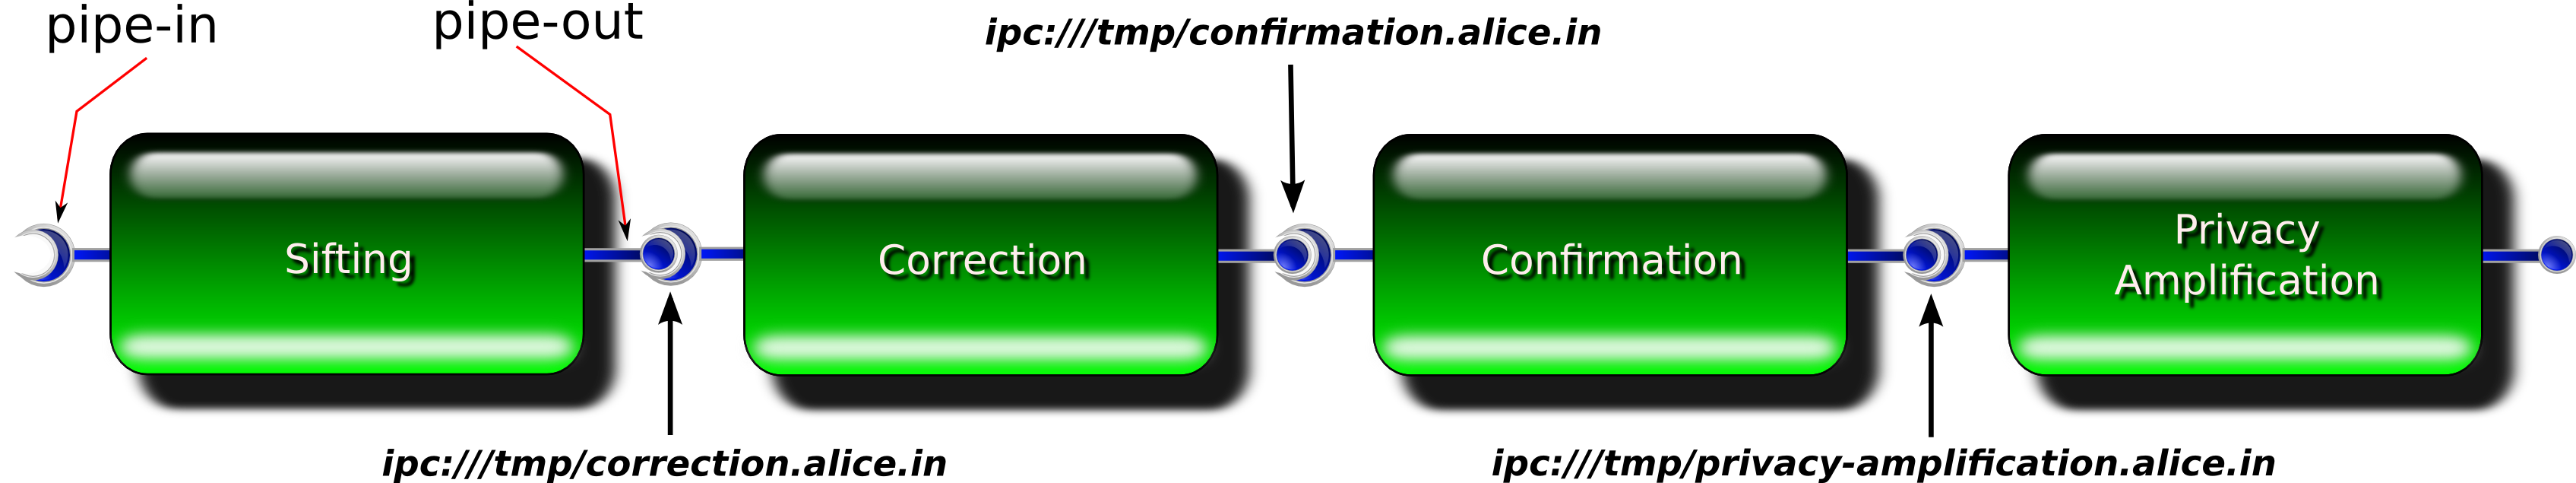
\includegraphics[scale=0.50,keepaspectratio=true]{./gfx/qkd-pipeline.png}
    \caption{An AIT QKD Pipeline.}
    \label{fig:qkd-pipeline}
\end{figure}

Figure \ref{fig:qkd-pipeline} shows a small pipeline at Alice's side. The keys here are generate inside the ``sifting'' QKD Module. This module's pipe-out is set to \texttt{ipc:///tmp/correction.alice.in} which, in turn, is the pipe-in of the next module ``correction''. This module pushes the corrected keys into \texttt{ipc:///tmp/confirmation.alice.in} where the keys are picked by the "confirmation" module. Once this module finished its work it is time to pass on the keys at \texttt{ipc:///tmp/privacy-amplification.alice.in} for the next module "privacy amplification".

\medskip

The addresses are provided as URLs\footnote{Uniform Resource Locator see \url{http://en.wikipedia.org/wiki/Url}}. Table \ref{tab:QKD Module pipe-in and pipe-out address schemes} lists all possible variations. When setting up a QKD pipeline you are free to switch connections techniques at will.

\begin{table}[h!]
    \begin{tabular}{llp{8cm}}
    Scheme                  &   Read/Write                              &   Example \\
    \hline
    \\
    \emph{empty}            &   \texttt{pipe\_in}/\texttt{pipe\_out}    &                                   \\ [0.7em]   
    & \multicolumn{2}{p{11cm}}{If the input address of the module has been left empty, then the module always creates a new fresh zero-length key to process. This might be initially used to create key structures based on values derived from the QKD hardware. If this is assigned to the output address then the key is discarded.} \\ [0.7em]    
    \\
    \texttt{stdin://}       &   \texttt{pipe\_in} only                  &  "\texttt{stdin://}"                \\ [0.7em]   
    & \multicolumn{2}{p{11cm}}{Read keys from \texttt{stdin} the standard UNIX input file descriptor.}\\ [0.7em]    
    \\
    \texttt{stdout://}      &   \texttt{pipe\_out} only                 &  "\texttt{stdout://}"               \\ [0.7em]
    & \multicolumn{2}{p{11cm}}{Write keys to \texttt{stdout} the standard UNIX output file descriptor.}\\ [0.7em]    
    \\
    \texttt{ipc://FILE}     &   \texttt{pipe\_in}/\texttt{pipe\_out}    &  "\texttt{ipc:///tmp/mod.in}"       \\ [0.7em]
    & \multicolumn{2}{p{11cm}}{Read and/or write keys from/to an interprocess communication port. This IPC port is labeled with FILE. This is the fastest way to interconnect two modules and is recommended.}\\ [0.7em]    
    \\
    \texttt{ipc://*}        &   \texttt{pipe\_in}/\texttt{pipe\_out}    &  "\texttt{ipc://*}"                 \\ [0.7em]
    & \multicolumn{2}{p{11cm}}{This is the same as \texttt{ipc://FILE} but this time the AIT QKD framework creates a new FILE address label for the interprocess communication port. The user has to query the address afterwards to figure out which concrete address has been chosen.}\\ [0.7em]    
    \\
    \texttt{tcp://IP:PORT}  &   \texttt{pipe\_in}/\texttt{pipe\_out}    &  "\texttt{tcp://172.20.30.54:7778}" \\ [0.7em]
    & \multicolumn{2}{p{11cm}}{Read and/or write keys from/to a TCP/IP socket.}\\ [0.7em]    
    \\
    \texttt{tcp://*:PORT}   &   \texttt{pipe\_in}/\texttt{pipe\_out}    &  "\texttt{tcp://*:7778}"            \\ [0.7em]
    & \multicolumn{2}{p{11cm}}{Read and/or write keys from/to a TCP/IP socket bound to \textbf{all} current interfaces. Hence: this is highly ambiguous and insecure and should be avoided.}\\ [0.7em]    
    \\
    \end{tabular}
    \caption{QKD Module \texttt{pipe\_in} and \texttt{pipe\_out} address schemes}
    \label{tab:QKD Module pipe-in and pipe-out address schemes}
\end{table}

\medskip

A totally valid example could be:

\begin{enumerate}

\item Start the QKD pipeline with a hardware depend module. Naturally this module will set its \texttt{pipe\_in} empty, since it the first one. As a consequence the QKD Module threads starts creating empty keys immediately. This empty keys can be filled with Quantum Events derived from the machines.

\item This hardware related module may now push its keys to an address called "\texttt{ipc:///sifting.in}". This is set as \texttt{pipe\_out} of the hardware module, but also as \texttt{pipe\_in} of the sifting module.

\item The sifting module picks up the key data at "\texttt{ipc:///sifting.in}" and exchanges sifting reconciliation data with its peer. Afterwards it pushes the sifted key to "\texttt{tcp://192.168.45.12:5231}" which has been set as \texttt{pipe\_out}. 

\item At the machine with the IP 192.168.45.12 a QKD Module listens on port 5231 (that is: \texttt{pipe\_in} has been set to "\texttt{tcp://192.168.45.12:5231}"). This machine has vast computational powers to run a sophisticated error correction algorithm. When this is done the machine pushed the key to "\texttt{tcp://192.168.45.67:1102}" (\texttt{pipe\_out}).

\item At 192.168.45.67 yet again another part of this QKD pipeline is run. At port 1102 (\texttt{pipe\_in} = "\texttt{tcp://192.168.45.67:1102}"), maybe confirmation. This confirmation pushes it keys to "\texttt{stdout://}".

\item The next module (privacy amplification) has been started with a single command line together with the confirmation previously: \texttt{\$ confirmation | privacy\_amplification}. From this line, it should be clear that the privacy amplification module's \texttt{pipe\_in} is set to "\texttt{stdin://}".

\end{enumerate}

Agreed, this is a pretty wild example, since pipe-URL schemes are mixed right within the pipeline. Even more: we switch even machines. With the \texttt{tcp://} scheme you may even run key reconciliation across the Internet. If you seek a challenge for confusion, you've found it by intermixing modules In- and Out- address URL schemes. As an advice: stick to the \texttt{ipc://FILE} scheme with concrete addresses as the FILE part.

\vspace{2cm}

\begin{center}
\begin{minipage}{10cm}
\textbf{Beware}: when passing the key data from one module to the next module within the pipeline you pass along also the cryptographic context. Having this cryptographic context at hand any malicious attacker has the ability to tamper key integrity. Passing key data to not authentic machines or modules is a severe security breach.
\end{minipage}
\end{center}

\vspace{2cm}

\subsection{Send and Receive Reconciliation data}
\label{subsec:Send and Receive Reconciliation data}

Sending and receiving reconciliation data involves having an Alice module (see "Module Roles" - section \ref{subsec:Module Roles}) connecting a remote Bob module. This is pretty likewise achieved as interconnecting QKD Modules to form a pipeline. Table \ref{tab:QKD Module peer-connect and peer-listen address schemes} lists possible address schemes for remote module communication.

\medskip

However here the more familiar client-server approach prevails. Bob always acts as a server and opens up a listening facility at \texttt{peer\_listen}. Alice in turn sets exactly this address as its \texttt{peer\_connect}. If there is either one of these the module is said to be "paired", although the module may not be connected (yet).

\medskip

Another difference is the fact that the message content exchanged is undefined. Every QKD Module has its own protocol for QKD post processing and therefore may implement any arbitrary message passing structures within.

\medskip

So the AIT QKD framework does not impose and data format on this connection. On the other hand the AIT QKD framework \emph{does} enforces security of messages when it comes to authenticity (see section \ref{subsec:Post Processing Authentication}).

\begin{table}[h]
    \begin{tabular}{lp{11cm}}
    Scheme                  &   Example \\
    \hline
    \\
    \texttt{tcp://IP:PORT}  &   \texttt{tcp://172.20.30.54:7778} \\ [0.7em]
    & Send and/or receive reconciliation data to/from a TCP/IP socket. This is the recommended scheme for remote communication.\\ [0.7em]    
    \\
    \texttt{tcp://*:PORT}   &   \texttt{tcp://*:7778}            \\ [0.7em]
    & Send and/or receive reconciliation data to/from a TCP/IP socket bound to \textbf{all} current interfaces. Hence: this is highly ambiguous and insecure and should be avoided.\\ [0.7em]    
    \\
    \texttt{ipc://FILE}     &   \texttt{ipc:///tmp/mod.in}       \\ [0.7em]
    & Send and/or receive reconciliation data to/from an interprocess communication port. This IPC port is labeled with FILE. This works only if the local and the "remote" machine are on the same system.\\ [0.7em]    
    \\
    \texttt{ipc://*}        &   \texttt{ipc://*}                 \\ [0.7em]
    & This is the same as \texttt{ipc://FILE} but this time the AIT QKD framework creates a new FILE address label for the interprocess communication port. The user has to query the address afterwards to figure out which concrete address has been chosen.\\ [0.7em]    
    \\
    \end{tabular}
    \caption{QKD Module \texttt{peer\_connect} and \texttt{peer\_listen} address schemes}
    \label{tab:QKD Module peer-connect and peer-listen address schemes}
\end{table}


\subsection{Key Synchronization}
\label{subsec:Key Synchronization}

The AIT QKD team tries its best to get the AIT QKD Modules functional and working. But bugs and errors will remain. Next, users are free to combine any QKD Modules created by other parties for special tasks right into their QKD pipelines.

\medskip

Buggy modules may drop a key every now and then, hang or simply leave the operating system's process space pretty spontaneously\footnote{in other words: they crash.} ... and there is the matter of possible parallelism of stochastic algorithms which may as well create an indeterministic sequence of keys as input for the next QKD Module. QKD Modules have to cope with incidents like this: key reordering and key dropping by a previous module.

\medskip

That's why there is key synchronization: when key synchronization is turned on and the QKD Module is paired and does have a non-void input pipe-in, incoming keys are placed into a set of out-of-sync keys.

\medskip

When looking for new keys to process the total set of the internal out-of-sync key-ids are compared with the peer module. Every match identified is transfered into an internal in-sync-FIFO-buffer\footnote{First-In-First-Out}. From this internal in-sync buffers keys are withdrawn and processed until empty.

\medskip

The keys in the out-of-sync buffer for which remote presence has not yet been confirmed will slowly cease as a TTL\footnote{Time To Live} is applied to them. Every time a synchronization attempt is run the TTL value is decreased. When it drops to 0, the key is deleted. This synchronization attempt is run every time a new key arrives or at least every second as a minimum.

\begin{figure}[h]
    \centering
    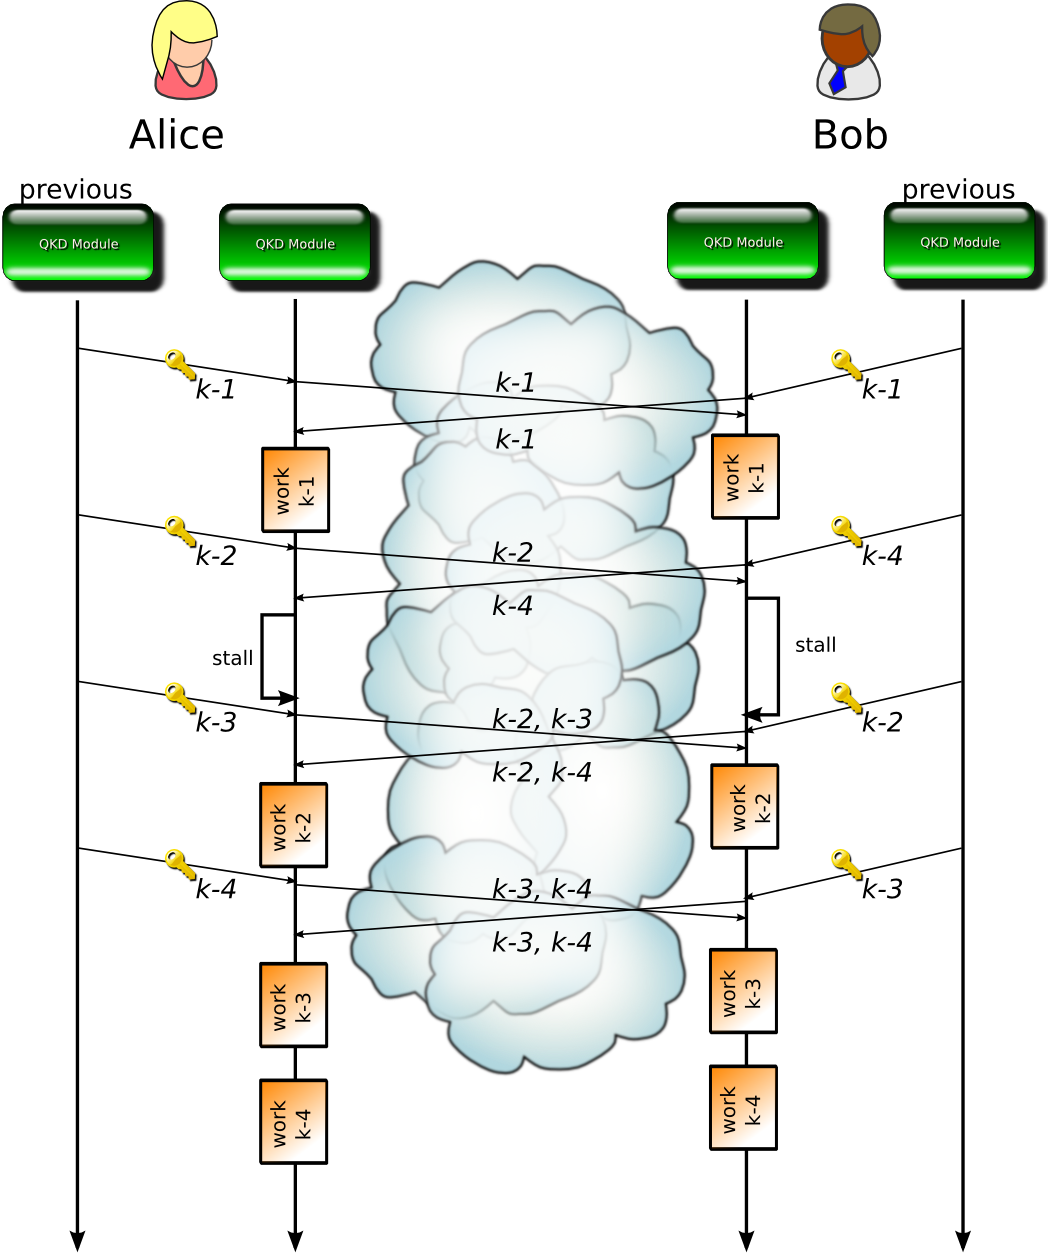
\includegraphics{./gfx/qkd-key-synchronization.png}
    \caption{Key Synchronization.}
    \label{fig:qkd-key-synchronization}
\end{figure}

\medskip

In figure \ref{fig:qkd-key-synchronization} a scenario is depicted. At the left side two Alice modules are shown whereas at the right side the corresponding remote peer Bob modules are drawn. At the outermost side the previous module for each is present. This previous module spills out keys in an unordered sequence. In the figure the sequence of keys at the Alice side is $k_1$, $k_2$, $k_3$ and $k_4$. At Bob's side it is: $k_1$, $k_4$, $k_2$ and $k_3$ having $k_4$ intermingled.

\medskip

Whenever the modules read a key or at least every second the list of present out-of-sync keys is transmitted to the peer. As both do the same, the list of current keys is awaited at every key processing start.

\medskip

In the sample all is ok for $k_1$. However at the very next step Alice gets $k_2$ and Bob $k_4$. As both parties do not share the same key to work on they are stalled until the next key arrives from the previous module (or a second passed). The very next key is $k_3$ at Alice's and $k_2$ at Bob's. They exchange out-of-sync key information and now detect that they do share at least key $k_2$.

\medskip

After finished working on $k_2$ and the very next key has been read Alice transmits $k_3$ and $k_4$ to Bob who does likewise. Now, both have two keys set in their in-sync FIFO on which they both start immediately to work on.

\medskip

Beware: this exchange of information does support stability of the QKD pipeline, yes, but this does not come without some drawbacks:

\begin{enumerate}

\item First, this additional exchange of messages is done in parallel. However, the arrival of the peer's out-of-sync keys identifiers is waited upon and thus could slow down overall QKD pipeline performance.

\item And more important: this syncing of keys are not bound to a key itself and therefore lacks an authentication context. Resulting in the fact that this sequence of out-of-sync keys is currently not authenticated. Up to this date it is currently not known if this could have a more severe impact than a simple Denial-of-Service attack\footnote{DoS: which sometimes impossible to prevent, e.g. simply cutting the fiber between Alice and Bob.}.

\end{enumerate}


\subsection{Post Processing Authentication}
\label{subsec:Post Processing Authentication}

QKD post processing has to be authentic to some extend. Within the AIT QKD R10 authentication checks are bound to processed keys.

\medskip

Whenever data is exchanged between Alice and Bob the reconciliation data crosses a potentially hostile environment. Messages can be altered or dropped. To mitigate such attacks incoming and outgoing messages are authenticated. As QKD aims for information theoretical security the authentication algorithms used must share this trait. Standard computational security as it is provided by common algorithms today like SHA is considered insufficient.

\medskip

As of writing no none key consuming authentication algorithm of information theoretical security is known. This is cause to a dilemma: 

\vspace{1cm}

\begin{center}
\begin{minipage}{10cm}
\shadowbox{
\begin{minipage}{9cm}
In order to create shared secret (quantum) keys with information theoretical security QKD post processing messages exchanged by the peers have to authentic.
\\ [0.5cm]
In order to authenticate the QKD post processing messages exchanged by the peers you have to apply already shared secret (quantum) keys.
\end{minipage}
}
\end{minipage}    
\end{center}

\vspace{1cm}

Hen or egg. Next, every authentication step consumes keys and with respect to the algorithms available they do so with a minimum consumption of key material each round. When authenticating every message the amount of keys consumed may exceed the key material produced by this step.

\medskip

\clearpage

The AIT QKD framework now implements \emph{delayed} authentication: 

\begin{enumerate}

\item Initialize an empty authentication contexts for each key: one for incoming messages, one for outgoing messages.

\item Whenever messages are exchanged, the message content is pushed on top of the authentication context: incoming messages on top of the incoming authentication context, outgoing messages on top of the outgoing context.

\item After a series of message has been exchanged and/or when a milestone within the post processing protocol has been reach (e.g. the final shared key is ready) both authentication contexts are finalized and the resulting authentication tags are compared with the peer.

\item If both tags result equal then the communication generating the depended key is considered authentic. If not the key is tampered and an attack likely.

\end{enumerate}

Authentication tag exchange itself is not authenticated. An adversary may alter these authentication tag comparison messages and would create yet another DoS\footnote{Denial of Service} attack since the key is dropped and an administrator been alarmed.

\medskip

Authentication contexts are now passed along the key from one module to another in the pipeline. This is done by serialization of the context and placing this serialized data into the key's meta data. As the serialization is done to create a stringified, human-readable version of the cryptographic context, this one is also used as initialization input to these contexts.

\medskip

A stringfied version of a cryptographic context is called a cryptographic \emph{scheme} string. The scheme string consists of 4 parts:

\medskip

\begin{center}
ALGORITHM[-VARIANT][:INITIAL\_KEY[:CURRENT\_STATE]]
\end{center}

\medskip

\begin{itemize}

\item{ALGORITHM}: this labels the algorithm used. Current valid algorithms are "evhash", "umac", "xor" and "null".

\item{VARIANT}: this indicates the algorithm variant, like "96" in "evhash-96" describing an Evaluation Hash generating 96 bit tags.

\item{INITIAL\_KEY}: this is the initial key used in hexadecimal.

\item{CURRENT\_STATE}: this is the current state of the cryptographic context.

\end{itemize}

\medskip

\noindent Example:

\begin{minipage}{0.9\textwidth}
\bigskip
\begin{verbatim}
evhash-96:02cc942de299:f4b0d86ffd53
\end{verbatim}
\medskip
\end{minipage}

This scheme describes an evaluation hash generating 96 bits with 0x02cc942de299 as input key and 0xf4b0d86ffd53 as current state of the authentication context.

\medskip

\noindent Example:

\begin{minipage}{0.9\textwidth}
\bigskip
\begin{verbatim}
xor
\end{verbatim}
\medskip
\end{minipage}

This scheme declares a xor cryptographic context. The xor-context is \emph{not} the periodic xor encryption but rather to full length encryption using a key with the same length of the original message.

\medskip

\clearpage

\noindent Example:

\begin{minipage}{0.9\textwidth}
\bigskip
\begin{verbatim}
null
\end{verbatim}
\medskip
\end{minipage}

This is the NULL-context. A context providing all internal cryptographic methods but calculating no tag or cypher at all.

\medskip

In order to provide authentication to the QKD post processing a dedicated module has been implemented: \texttt{qkd-auth} see section \ref{subsec:qkd-auth}. By utilizing this module you have to ability to assign each key in the QKD pipeline a new initial key which will be used to authenticate the messages exchanged in the QKD post processing pipeline to ensure a shared secret key.

\medskip

\begin{figure}[h]
    \centering
    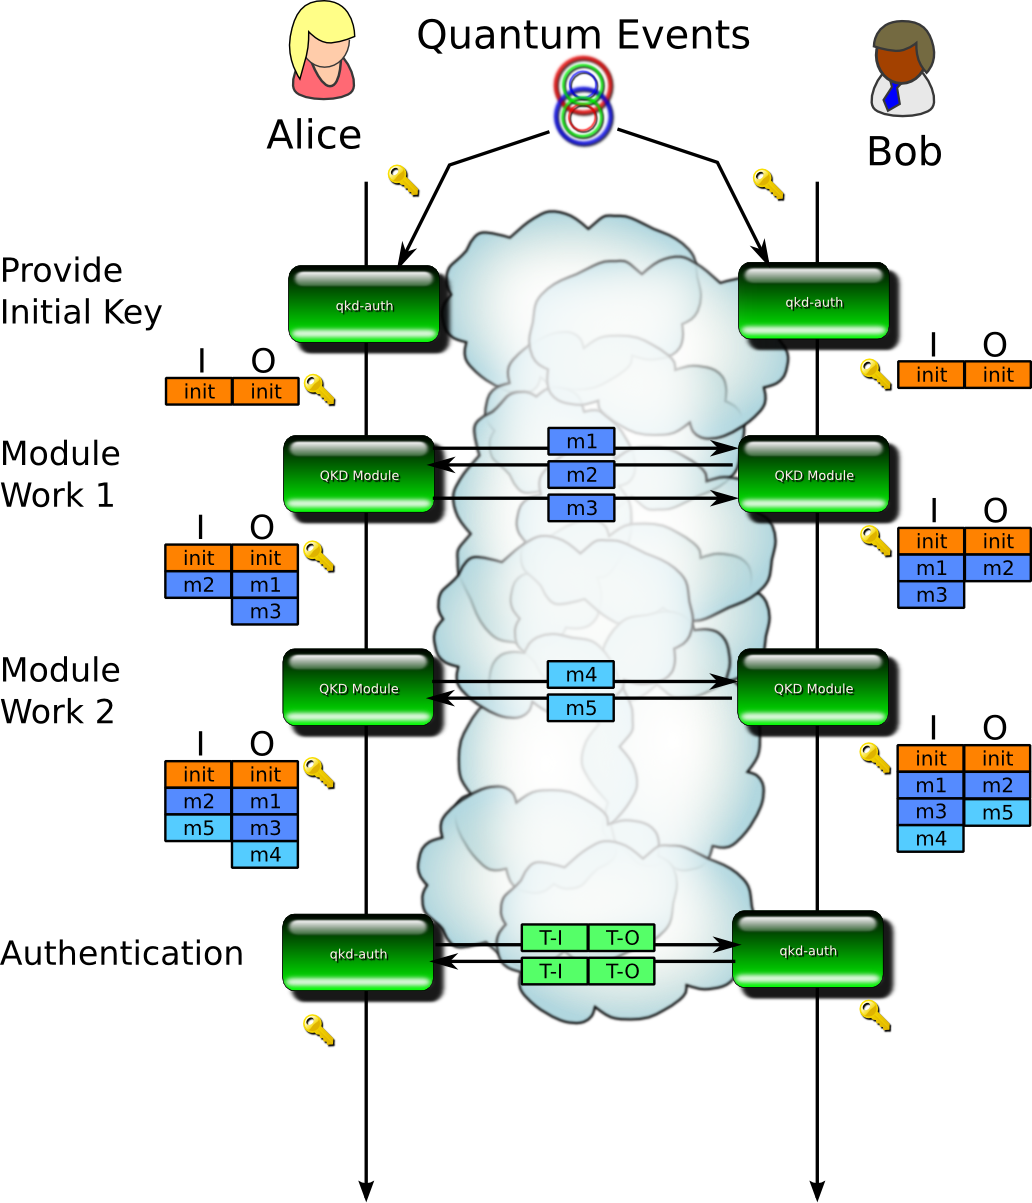
\includegraphics{./gfx/qkd-stack-authentication.png}
    \caption{AIT QKD Stack Authentication.}
    \label{fig:qkd-stack-authentication}
\end{figure}

Figure \ref{fig:qkd-stack-authentication} summarizes the ideas. At first quantum events are picked which form the basis of the would-be shared secret key. At the next step the \texttt{qkd-auth} module creates an incoming and an outgoing cryptographic context and provides the initial secret keys for both.

\medskip

As the key is passed along the QKD post processing pipeline more and more exchanges messages are ``stacked'' upon the cryptographic contexts. In the figure the very next module exchanges $m_1$, $m_2$ and $m_3$ and then passes the key to next module in the pipeline. The latter in turn adds $m_4$ and $m_5$ as exchanged messages to the cryptographic contexts.

\medskip

Finally the \texttt{qkd-auth} module receives the key, creates the incoming and outgoing authentication tags $T_I$ and $T_O$ and compares these values with the peer's. On equality the key is passed along to the next module.


\subsection{Module Configuration}
\label{subsec:Module Configuration}

Each module has a standard set of configuration options. The main and recommended way applying values to these options is by loading a configuration file. But all configuration options are also available on the DBus (see section \ref{subsec:Module DBus Interaction}).

\medskip

Note that some options have different effect whether the module is started as Alice or as Bob. Therefore the module's role assignment \emph{must} be set in advance. This role assignment along with the debug options is usually passed on the command line during process invocation. The AIT tries to minimize the arguments on the command line and put an emphasis on configuration files. These files may be loaded any time during operation to reapply the configuration values again.

\medskip

The configuration files are of the well known INI-Syntax files:

\begin{itemize}

\item Each empty line is ignored.

\item Each line starting with a \texttt{\#} is a comment.

\item A single word enclosed in square brackets like \texttt{[module]} starts a new section.

\item Each line is composed as \texttt{key = value} assigning a value to a key in a section.

\end{itemize}

\medskip

Section names solely serve as a way to organize the configuration file in a more human friendly manner. Effectively, each key name is prefixed with the section name (without the brackets). Dots "\texttt{.}" are used as separator. More than one QKD Module can be configured with a single configuration file. To distinguish entries each module picks its keys if they match a fixed \texttt{module.} prefix and the modules id at beginning of the module's key. Table \ref{tab:Standard QKD Module configuration keys} lists the standard module key entries.

\medskip

\begin{table}[h]
    \begin{tabular}{lp{8cm}}
    Name                                    &   Description \\
    \hline
    \\
    module.\emph{id}.alice.url\_peer        &   This is the address which is Alice going to connect to, if the module is started as Alice. \\[0.7em]
    module.\emph{id}.alice.url\_pipe\_in    &   This is the pipe-in address of the module, if the module is started as Alice. \\[0.7em]
    module.\emph{id}.alice.url\_pipe\_out   &   This is the pipe-out address of the module, if the module is started as Bob. \\[0.7em]
    module.\emph{id}.bob.url\_listen        &   The address at which the Bob module is going to listen for Alice's connection attempts. \\[0.7em]
    module.\emph{id}.bob.url\_pipe\_in      &   The pipe-in address if the module is started as Bob. \\[0.7em]
    module.\emph{id}.bob.url\_pipe\_out     &   The pipe-out address if the module is started as Bob. \\[0.7em]
    module.\emph{id}.pipeline               &   The name of the pipeline the module participates. \\[0.7em]
    module.\emph{id}.random\_url            &   The address if the random values character device this module ought to use. \\[0.7em]
    module.\emph{id}.synchronize\_keys      &   If set to "true", "on" or "1" the module does key synchronization see section \ref{subsec:Key Synchronization}. \\[0.7em]
    module.\emph{id}.synchronize\_ttl        &   TTL for out-of-sync keys if key synchronization is turned on. \\[0.7em]
    \end{tabular}
    \caption{Standard QKD Module configuration keys}
    \label{tab:Standard QKD Module configuration keys}
\end{table}

\medskip

\clearpage

Listing \ref{lst:module-configuration-example} shows a segment of a configuration file for modules. The lines 1, 5, and 17 are ignored since they start with an \texttt{\#}. The lines 2, 4, and 16 are empty and ignored too.

\begin{lstlisting}[language=,numbers=left,xleftmargin=1cm,frame=lines,caption={Module Configuration Example},label=lst:module-configuration-example]
# this is a comment (and ignored)

[module]

# bb84 module configuration
bb84.alice.url_peer = tcp://192.168.137.12:7120
bb84.alice.url_pipe_in = ipc:///tmp/bb84.alice.in
bb84.alice.url_pipe_out = ipc:///tmp/cascade.alice.in
bb84.bob.url_listen = tcp://192.168.137.12:7120
bb84.bob.url_pipe_in = ipc:///tmp/bb84.bob.in
bb84.bob.url_pipe_out = ipc:///tmp/cascade.bob.in
bb84.pipeline = default
bb84.synchronize_keys = true
bb84.synchronize_ttl = 10
bb84.rawkey_length = 1024

# cascade module configuration
cascade.alice.url_peer = tcp://192.168.137.12:7140
cascade.alice.url_pipe_in = ipc:///tmp/cascade.alice.in
cascade.alice.url_pipe_out = stdout://
cascade.bob.url_listen = tcp://192.168.137.12:7140
cascade.bob.url_pipe_in = ipc:///tmp/cascade.bob.in
cascade.bob.url_pipe_out = stdout://
cascade.synchronize_keys = true
cascade.synchronize_ttl = 10
cascade.pipeline = default
\end{lstlisting}

\medskip

\begin{itemize}

\item Line 3 now starts the "module" section. All keys are now prefixed with the "module" keyword, e.g. yielding line 6 now really been "module.bb84.alice.url\_peer".

\item Lines 6 up to 15 now configure the BB84 module. The very first six lines of this module configuration now deal with the pipe-in, pipe-out and remote connection settings for Alice and Bob respectively. Whenever a module is instantiated as Alice it picks its settings accordingly and vice versa as Bob. 

\item As you can see, the setting \emph{bb84.alice.url\_peer} (line 6) does match \emph{bb84.bob.url\_listen} (line 9). This enables the Alice and Bob modules to locate each other in the network. This is how remote peer connection is configured.

\item The lines 7 and 8 for Alice and 10 and 11 for Bob do configure the addresses \emph{within} the pipeline. Adjusting these lines is how a QKD pipeline is created see section \ref{subsec:Reading and Writing QKD keys}. When looking closely you see, that the output of the BB84 module does exactly match the input of the next module below: Alice's BB84 output (line 8) is set to Alice's Cascade input (line 19).

\item Lines 20 and 23 direct the output of the Cascade to be \texttt{stdout}. This will dump the corrected keys to the stdout UNIX file descriptor which can be redirected into a file on disk.

\item Both modules do enable key synchronization (lines 13, 14 and lines 24, 25). There is no dedicated "alice" or "bob" keyword within the key's name, so this key is used for both modules roles. 

\item The pipeline's name of both modules is set to "default".

\item The BB84 knows of a non standard module configuration which is unique to this module: "rawkey\_length". This key describes the minimum length of a sifted key in bytes. However, the Cascade module lacks such key. This is a hint to the fact, that each module may introduce new arbitrary options.

\end{itemize}

\medskip

As any module is free to implement any new configuration parameter, these options have to be studied alongside at the discussion of each module (see section \ref{sec:AIT QKD Module Menagerie}).

\medskip

The recommend way to configure the QKD system is now to setup a single QKD configuration file having entries for all participating modules. This file is now the value to the \texttt{--config} option on the command line for each module in combination with a \texttt{--bob} flag, if the module is started as Bob.


\subsection{Module DBus Interaction}
\label{subsec:Module DBus Interaction}

Each AIT QKD Module offers a rich set of variables on the DBus. The DBus is a modern IPC technique used in today's Linux and UNIX systems. Processes freely advertise properties and methods on the DBus to be called by any other process running on the same machine.

\medskip

The AIT QKD framework uses this de-facto standard to publish the module's states and methods. Administrative tasks and analyses of system behavior can be done with any tools capable connecting to the DBus.

\medskip

The AIT recommends two tools for this:

\begin{enumerate}

\item For ease of access the \texttt{qdbusviewer}\footnote{Debian provides this application in the \texttt{qt-dev-tools} package.}. This one lets a user view the DBus with the help of a graphical user interface (GUI) as shown in figure \ref{fig:qkd-dbus-viewer}.

\item Fast access and usage within administrative bash-scripts is done with \texttt{qdbus}\footnote{On Debian derived system this is found in the \texttt{qdbus} package.}.

\end{enumerate}

\medskip

Note, there are many more DBus related packages available for the user's problem and/or flavor.

\begin{figure}[h]
    \centering
    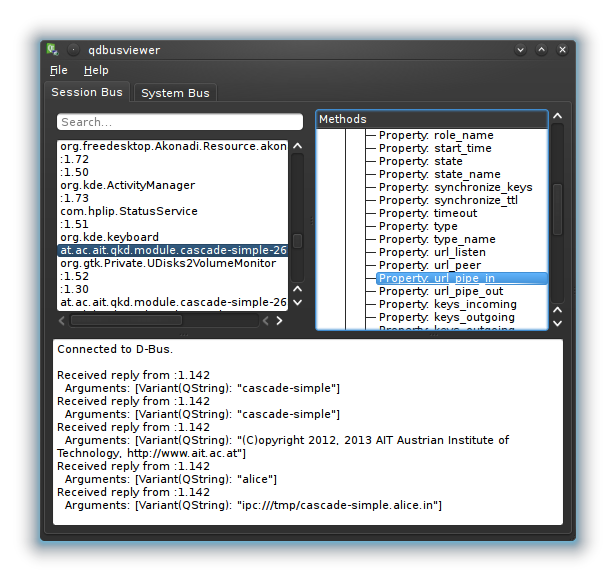
\includegraphics[scale=0.8,keepaspectratio=true]{./gfx/qkd-dbus-viewer.png}
    \caption{\texttt{qdbusviewer} examining the QKD "Cascade" module.}
    \label{fig:qkd-dbus-viewer}
\end{figure}

\medskip

Addressing a QKD Module on the DBus is simple: each QKD Module has a unique name which is composed by the prefix ``at.ac.ait.qkd.module.'' and the module id followed by a dash and the process id, e.g. ``at.ac.ait.qkd.module.cascade-simple-28991''. Each module has a root ``/Module'' path element which offers all properties and methods. Table \ref{tab:QKD Module DBus Properties} lists the module's DBus Properties, table \ref{tab:QKD Module DBus Methods}.

\medskip

\begin{table}[h!]
    \begin{tabular}{lcp{8cm}}
    Name                        &   Accessibility       &   Description \\
    \hline
    \\
    debug                       &   Read/Write          &   Enable/Disable debug output on stderr.\\
    hint                        &   Read/Write          &   An arbitrary text which helps to identify and interconnect modules.\\
    id                          &   Read Only           &   ID of the module.\\
    description                 &   Read Only           &   Description of the module.\\
    disclosed\_bits\_incoming   &   Read Only           &   Total number of disclosed bits the module received so far in all keys (via pipe-in).\\
    disclosed\_bits\_incoming   &   Read Only           &   Total number of disclosed bits the module sent so far in all keys (via pipe-out).\\
    error\_bits\_incoming       &   Read Only           &   Total number of error bits the module received so far in all keys (via pipe-in).\\
    error\_bits\_outgoing       &   Read Only           &   Total number of error bits the module sent so far in all keys (via pipe-out).\\
    key\_bits\_incoming         &   Read Only           &   Total number of key bits the module received so far (via pipe-in).\\
    key\_bits\_outgoing         &   Read Only           &   Total number of key bits the module sent so far (via pipe-out).\\
    keys\_incoming              &   Read Only           &   Total number of keys the module received so far (via pipe-in).\\
    keys\_outgoing              &   Read Only           &   Total number of keys the module sent so far (via pipe-out).\\
    organisation                &   Read Only           &   Organisation/Institute/Company of module.\\
    paired                      &   Read Only           &   Module has a peer module (but maybe not connected).\\
    process\_id                 &   Read Only           &   PID of the module process within the operating system.\\
    process\_image              &   Read Only           &   Full path to the module program.\\
    random\_url                 &   Read/Write          &   The random URL used to gain random values inside the module.\\
    role                        &   Read/Write          &   The role the module inhabits (0 = Alice, 1 = Bob).\\
    start\_time                 &   Read Only           &   UNIX epoch timestamp of module launch.\\
    state                       &   Read Only           &   Current state of the module (see section \ref{subsec:Module States}).\\
    state\_name                 &   Read Only           &   Human readable string describing the module state.\\
    synchronize\_keys           &   Read/Write          &   Synchronize key-ids with remote peer module before processing.\\
    synchronize\_ttl            &   Read/Write          &   TTL for not out-of-sync keys.\\
    timeout                     &   Read/Write          &   Number of milliseconds to wait after a failed read (from pipe-in).\\
    type                        &   Read Only           &   Type of the module (Sifting, Error Correction, etc ...).\\
    type\_name                  &   Read Only           &   Human readable description of the module type.\\
    url\_listen                 &   Read/Write          &   URL for peer (Bob serving endpoint).\\
    url\_peer                   &   Read/Write          &   URL of a remote module this instance connects to (Alice).\\
    url\_pipe\_in               &   Read/Write          &   URL of incoming Pipe (serving endpoint).\\
    url\_pipe\_out              &   Read/Write          &   URL of outgoing Pipe.\\
    \end{tabular}
    \caption{QKD Module DBus Properties}
    \label{tab:QKD Module DBus Properties}
\end{table}

\medskip

\begin{table}[ht!]
    \begin{tabular}{lp{9cm}}
    Name                                                &   Description \\
    \hline
    \\
    pause()                                             &   If the module is in the RUNNING state the module switches back to READY.\\ [0.5em]
    resume()                                            &   This is the opposite call to pause(): switch into the RUNNING state.\\ [0.5em]
    run(\emph{pipe-in}, \emph{pipe-out}, \emph{peer})   &   Sets the module into the READY state. The given arguments are the URL of pipe-in, pipe-out and peer (or listen when called Bob). These are optional. If left blank the already configured settings are used.\\ [0.5em]
    synchronize()                                       &   This method triggers a key synchronization attempt. This is additional to the already internally used timeouts.\\ [0.5em]
    terminate()                                         &   Shutdown the module.\\ [0.5em]
    \end{tabular}
    \caption{QKD Module DBus Methods}
    \label{tab:QKD Module DBus Methods}
\end{table}

\medskip

Using \texttt{qdbus} to query the total of all error bits so far detected (and corrected) by a running cascade instance is done as depicted in listing \ref{lst:querying-the-dbus-with-qdbus}. Calling \texttt{qdbus} only with the object and the path (``/Module'') as in the first line does simply list all available properties, methods and signals. The last but one line now does queries the ``error\_bits\_outgoing'' value, which returns 52560.

\begin{lstlisting}[language=,numbers=none,frame=lines,caption={Querying the DBus with qdbus},label=lst:querying-the-dbus-with-qdbus]
$ qdbus at.ac.ait.qkd.module.cascade-simple-28991 /Module
property readwrite bool at.ac.ait.qkd.module.debug
property read QString at.ac.ait.qkd.module.description
property read qulonglong at.ac.ait.qkd.module.disclosed_bits_incoming
property read qulonglong at.ac.ait.qkd.module.disclosed_bits_outgoing
property read qulonglong at.ac.ait.qkd.module.error_bits_incoming
property read qulonglong at.ac.ait.qkd.module.error_bits_outgoing
property readwrite QString at.ac.ait.qkd.module.hint
...
method void org.freedesktop.DBus.Peer.Ping()
$ qdbus at.ac.ait.qkd.module.cascade-simple-28991 /Module 
                                                   error_bits_outgoing
52560
\end{lstlisting}

\medskip

Additional to the already mentioned properties and methods all QKD Modules also do signal their termination with the \texttt{terminated} event which can be trapped by others to react.

\clearpage


\section{AIT QKD Module Menagerie}
\label{sec:AIT QKD Module Menagerie}

This section lists the available AIT QKD modules along with their arguments and properties.

\medskip

Besides the mentioned extra properties and methods to each QKD Module all QKD Modules do share the configuration values declared in section \ref{subsec:Module Configuration} and the DBus interface as shown in section \ref{subsec:Module DBus Interaction}.

\medskip

The commonly shared arguments on the command line are:

\medskip

\begin{tabular}{lp{10cm}}

\texttt{--bob} or \texttt{-b}       & Set this instance to act as Bob. \\ [0.5em]
\texttt{--config} or \texttt{-c}    & URL to the configuration file. \\ [0.5em]
\texttt{--debug} or \texttt{-d}     & When set enables debug output on stderr immediately.\\ [0.5em]
\texttt{--help} or \texttt{-h}      & Shows a small help page. \\ [0.5em]
\texttt{--run} or \texttt{-r}       & Runs the QKD Module immediately (switches into RUNNING after configuration). \\ [0.5em]
\texttt{--version} or \texttt{-v}   & Shows QKD Module's implementation version. \\ [0.5em]

\end{tabular}

In the following each QKD Module is described alongside additional arguments to the command line, DBus properties and DBus methods. The ``Paired'' flag states if the QKD Module does need a remote peer module to interact with.

\clearpage


\subsection{qkd-auth}
\label{subsec:qkd-auth}

\textbf{Description}: This QKD Module does the authentication as described in section \ref{subsec:Post Processing Authentication}. This module acts twofold within a QKD pipeline:

\begin{enumerate}

\item When a key is read \textbf{and} the key has an associated cryptographic context which is not \texttt{null} then this module runs an authentication step. If successful the cryptographic context are set to \texttt{null} and the next phase follows. \\[1em] If the authentication fails the key is discarded and the logs are filled with a corresponding critical message.

\item If the authentication module does have an initial key to apply the bypassing key's cryptographic contexts are set up accordingly.

\end{enumerate}

The idea for this separation is to have an authentication start at the beginning of the QKD pipeline and finally an authentication check at end. The cryptographic contexts are initialized by providing a cryptographic scheme like ``\texttt{evhash-96:02cc942de299}''.

\medskip

If the authentication check has been successful the bypassing key is stored inside the QKD Module for the very next authentication or bypassed if the internal key storages are above a given threshold.

\bigskip

\noindent \textbf{Paired}: yes.

\bigskip

\noindent \textbf{Extra Commandline Options}: \emph{none}.

\bigskip

\noindent \textbf{Extra DBus Properties}: 

\medskip

\begin{tabular}{llp{7cm}}

Name                                & Accessibility &   Description \\
\hline
\\
\texttt{available\_keys\_incoming}  & Read Only     &   Current available key material for incoming final authentication. \\ [0.5em]
\texttt{available\_keys\_outgoing}  & Read Only     &   Current available key material for outgoing final authentication. \\ [0.5em]
\texttt{current\_scheme\_in}        & Read Only     &   The current incoming initial authentication scheme. \\ [0.5em]
\texttt{current\_scheme\_out}       & Read Only     &   The current outgoing initial authentication scheme. \\ [0.5em]
\texttt{next\_scheme\_in}           & Read/Write    &   The next incoming initial authentication scheme to use. \\ [0.5em]
\texttt{next\_scheme\_out}          & Read/Write    &   The next outgoing initial authentication scheme to use. \\ [0.5em]
\texttt{threshold}                  & Read/Write    &   Threshold of key material to reserve in bytes (IN and OUT). \\ [0.5em]

\end{tabular}

\bigskip

\noindent \textbf{Extra DBus Methods}: 

\medskip

\begin{tabular}{lp{10cm}}

Method                              & Description \\
\hline
\\
store\_keys\_incoming(\emph{blob})  & Add a memory block (blob) as incoming key material. \\ [0.5em]
store\_keys\_outgoing(\emph{blob})  & Add a memory block (blob) as outgoing key material. \\ [0.5em]

\end{tabular}

\bigskip

\clearpage

\noindent \textbf{Extra Configuration File Options}:

\medskip

\begin{tabular}{lp{9cm}}

Option                              & Description \\
\hline
\\
\texttt{alice.scheme.incoming}      & The scheme to use as Alice incoming. \\ [0.5em]
\texttt{alice.scheme.outgoing}      & The scheme to use as Alice outgoing. \\ [0.5em]
\texttt{bob.scheme.incoming}        & The scheme to use as Bob incoming. \\ [0.5em]
\texttt{bob.scheme.outgoing}        & The scheme to use as Bob outgoing. \\ [0.5em]
\texttt{alice.key.incoming}         & The key material used for final key operation. The value is given is taken as-is. \\ [0.5em]
\texttt{alice.key.outgoing}         & The key material used for final key operation. The value is given is taken as-is. \\ [0.5em]
\texttt{bob.key.incoming}           & The key material used for final key operation. The value is given is taken as-is. \\ [0.5em]
\texttt{bob.key.outgoing}           & The key material used for final key operation. The value is given is taken as-is. \\ [0.5em]

\end{tabular}

\bigskip

\noindent \textbf{Sample Configuration Section}: 

\medskip

\begin{lstlisting}[language=,numbers=none,frame=lines]
[module]
auth.alice.url_peer = tcp://*:7110
auth.alice.url_pipe_in = ipc:///tmp/auth_pre.alice.in
auth.alice.url_pipe_out = ipc:///tmp/bb84.alice.in
auth.bob.url_listen = tcp://*:7110
auth.bob.url_pipe_in = ipc:///tmp/auth_pre.bob.in
auth.bob.url_pipe_out = ipc:///tmp/bb84.bob.in
auth.pipeline = default
auth.synchronize_keys = true
auth.synchronize_ttl = 10
auth.alice.scheme.incoming = evhash-96:3979ea51296ee3a6e0ab4460
auth.alice.scheme.outgoing = evhash-96:5ce72a8a312ff5aa3316c37f
auth.bob.scheme.outgoing = evhash-96:5ce72a8a312ff5aa3316c37f
auth.bob.scheme.incoming = evhash-96:3979ea51296ee3a6e0ab4460
auth.alice.key.incoming = "This is a secret key B->A"
auth.alice.key.outgoing = "This is a secret key A->B"
auth.bob.key.incoming = "This is a secret key A->B"
auth.bob.key.outgoing = "This is a secret key B->A"
\end{lstlisting}

\clearpage


\subsection{qkd-bb84}
\label{subsec:qkd-bb84}

\textbf{Description}: This module runs the BB84 protocol. As this module ``generates'' the new key id in the first place this module applies the key-id to the generated key.

\medskip

As pipelines can be run in parallel and then merge into one single module somewhere down the line, for this merging module some precautionary measures have to be done in order not to mix up key-ids from two concurrent pipelines. This is when the key id pattern steps in.

\medskip

The key id pattern is a string holding a \emph{SHIFT} and a \emph{ADD} value (e.g. ``3/1''; $SHIFT = 3$ and $ADD = 1$). Whenever a new key-id is created an internal counter is incremented. This value is then shifted left by \emph{SHIFT} bits and finally the \emph{ADD}-value is added. With this technique one can ran $2^{SHIFT}$ parallel pipelines.

\bigskip

\noindent \textbf{Paired}: yes.

\bigskip

\noindent \textbf{Extra Commandline Options}: 

\medskip

\begin{tabular}{lp{10cm}}

Option                              & Description \\
\hline
\\
\texttt{--length} or \texttt{-l}    & Minimum length of the generated sifted key in bytes. \\ [0.5em]

\end{tabular}

\bigskip

\noindent \textbf{Extra DBus Properties}:

\medskip

\begin{tabular}{llp{7cm}}

Name                        & Accessibility &   Description \\
\hline
\\
\texttt{base\_ratio}        & Read Only     &   The 1-second moving average of the last base equality ratio. \\ [0.5em]
\texttt{current\_id}        & Read Only     &   The current key id we are sifting. \\ [0.5em]
\texttt{current\_length}    & Read Only     &   The current key length in bits we have sifted so far. \\ [0.5em]
\texttt{key\_id\_pattern}   & Read/Write    &   The key id pattern used for new keys (default: ``0/0''). \\ [0.5em]
\texttt{rawkey\_length}     & Read/Write    &   The minimum length of the raw key generated in bytes. \\ [0.5em]

\end{tabular}

\bigskip

\noindent \textbf{Extra DBus Methods}: \emph{none}.

\bigskip

\noindent \textbf{Extra Configuration File Options}:

\medskip

\begin{tabular}{lp{9cm}}

Option                      & Description \\
\hline
\\
\texttt{key\_id\_pattern}   & The key id pattern used for new keys (default: ``0/0''). \\ [0.5em]
\texttt{rawkey\_length}     & Minimum size of sifted key in bytes before forwarding. \\ [0.5em]

\end{tabular}

\bigskip

\clearpage

\noindent \textbf{Sample Configuration Section}: 

\medskip

\begin{lstlisting}[language=,numbers=none,frame=lines]
[module]
bb84.alice.url_peer = tcp://*:7120
bb84.alice.url_pipe_in = ipc:///tmp/bb84.alice.in
bb84.alice.url_pipe_out = ipc:///tmp/cascade-simple.alice.in
bb84.bob.url_listen = tcp://*:7120
bb84.bob.url_pipe_in = ipc:///tmp/bb84.bob.in
bb84.bob.url_pipe_out = ipc:///tmp/cascade-simple.bob.in
bb84.pipeline = default
bb84.synchronize_keys = true
bb84.synchronize_ttl = 10
bb84.key_id_pattern = 2/1
bb84.rawkey_length = 1024
\end{lstlisting}

\clearpage


\subsection{qkd-buffer}
\label{subsec:qkd-buffer}

\textbf{Description}: This module buffers incoming keys within the pipe up to a minimum size.

\bigskip

\noindent \textbf{Paired}: yes.

\bigskip

\noindent \textbf{Extra Commandline Options}: \emph{none}.

\bigskip

\noindent \textbf{Extra DBus Properties}:

\medskip

\begin{tabular}{llp{7cm}}

Name                        & Accessibility &   Description \\
\hline
\\
\texttt{cur\_key\_size}     & Read Only     &   Current key size (in bytes) for forward. \\ [0.5em]
\texttt{min\_key\_size}     & Read/Write    &   Minimum key size (in bytes) for forward. \\ [0.5em]

\end{tabular}

\bigskip

\noindent \textbf{Extra DBus Methods}: \emph{none}.

\bigskip

\noindent \textbf{Extra Configuration File Options}: 

\medskip

\begin{tabular}{lp{9cm}}

Option                      & Description \\
\hline
\\
\texttt{min\_key\_size}     & Minimum size of the buffered key before forwarding. \\ [0.5em]

\end{tabular}

\bigskip

\noindent \textbf{Sample Configuration Section}: 

\medskip

\begin{lstlisting}[language=,numbers=none,frame=lines]
[module]
buffer.alice.url_peer = tcp://*:7170
buffer.alice.url_pipe_in = ipc:///tmp/buffer.alice.in
buffer.alice.url_pipe_out = ipc:///tmp/privacy-amplification.alice.in
buffer.bob.url_listen = tcp://*:7170
buffer.bob.url_pipe_in = ipc:///tmp/buffer.bob.in
buffer.bob.url_pipe_out = ipc:///tmp/privacy-amplification.bob.in
buffer.pipeline = default
buffer.min_key_size = 10000
\end{lstlisting}

\clearpage


\subsection{qkd-cascade-simple}
\label{subsec:qkd-cascade-simple}

\textbf{Description}: This is the simple and naive Cascade error correction.

\bigskip

\noindent \textbf{Paired}: yes.

\bigskip

\noindent \textbf{Extra Commandline Options}: \emph{none}.

\bigskip

\noindent \textbf{Extra DBus Properties}: \emph{none}.

\bigskip

\noindent \textbf{Extra DBus Methods}: \emph{none}.

\bigskip

\noindent \textbf{Extra Configuration File Options}: \emph{none}.

\bigskip

\noindent \textbf{Sample Configuration Section}: 

\medskip

\begin{lstlisting}[language=,numbers=none,frame=lines]
[module]
cascade-simple.alice.url_peer = tcp://*:7140
cascade-simple.alice.url_pipe_in = ipc:///tmp/cascade-simple.alice.in
cascade-simple.alice.url_pipe_out = ipc:///tmp/confirmation.alice.in
cascade-simple.bob.url_listen = tcp://*:7140
cascade-simple.bob.url_pipe_in = ipc:///tmp/cascade-simple.bob.in
cascade-simple.bob.url_pipe_out = ipc:///tmp/confirmation.bob.in
cascade-simple.synchronize_keys = true
cascade-simple.synchronize_ttl = 10
cascade-simple.pipeline = default
\end{lstlisting}

\clearpage


\subsection{qkd-cat}
\label{subsec:qkd-cat}

\textbf{Description}: Read a key file and push the content into the QKD pipeline. This is for test and debug purpose.

\bigskip

\noindent \textbf{Paired}: no.

\bigskip

\noindent \textbf{Extra Commandline Options}:

\medskip

\begin{tabular}{lp{10cm}}

Option                            & Description \\
\hline
\\
\texttt{--file} or \texttt{-f}    & Key file to read. \\ [0.5em]
\texttt{--loop} or \texttt{-l}    & Loop key push. \\ [0.5em]

\end{tabular}

\bigskip

\noindent \textbf{Extra DBus Properties}:

\medskip

\begin{tabular}{llp{7cm}}

Name                    & Accessibility &   Description \\
\hline
\\
\texttt{file\_url}      & Read/Write    &   File URL to read from. \\ [0.5em]
\texttt{loop}           & Read/Write    &   Loop key push. \\ [0.5em]

\end{tabular}

\bigskip

\noindent \textbf{Extra DBus Methods}: \emph{none}.

\bigskip

\noindent \textbf{Extra Configuration File Options}: 

\medskip

\begin{tabular}{lp{9cm}}

Option                      & Description \\
\hline
\\
\texttt{alice.file\_url}    & URL of the file to read if run as Alice. \\ [0.5em]
\texttt{bob.file\_url}      & URL of the file to read if run as Bob. \\ [0.5em]
\texttt{loop}               & Loop file: ``true'' or ``false''. \\ [0.5em]

\end{tabular}

\bigskip

\noindent \textbf{Sample Configuration Section}: 

\medskip

\begin{lstlisting}[language=,numbers=none,frame=lines]
[module]
cat.alice.file_url = cat_keys.alice
cat.alice.url_pipe_out = ipc:///tmp/auth_pre.alice.in
cat.bob.file_url = cat_keys.bob
cat.bob.url_pipe_out = ipc:///tmp/auth_pre.bob.in
cat.pipeline = default
cat.loop = false
\end{lstlisting}

\clearpage


\subsection{qkd-confirmation}
\label{subsec:qkd-confirmation}

\textbf{Description}: This module runs the Confirmation after the Error Correction.

\bigskip

\noindent \textbf{Paired}: yes.

\bigskip

\noindent \textbf{Extra Commandline Options}:

\medskip

\begin{tabular}{lp{10cm}}

Option                              & Description \\
\hline
\\
\texttt{--rounds} or \texttt{-n}    & Number of rounds to run. \\ [0.5em]

\end{tabular}

\bigskip

\noindent \textbf{Extra DBus Properties}:

\medskip

\begin{tabular}{llp{7cm}}

Name                        & Accessibility &   Description \\
\hline
\\
\texttt{bad\_keys}          & Read Only     &   Absolute number of bad, unconfirmed keys so far. \\ [0.5em]
\texttt{confirmed\_keys}    & Read Only     &   Absolute number of confirmed keys so far. \\ [0.5em]
\texttt{rounds}             & Read/Write    &   Get or set the number of confirmation rounds. \\ [0.5em]

\end{tabular}

\bigskip

\noindent \textbf{Extra DBus Methods}: \emph{none}.

\bigskip

\noindent \textbf{Extra Configuration File Options}:

\medskip

\begin{tabular}{lp{9cm}}

Option                      & Description \\
\hline
\\
\texttt{rounds}             & Number of confirmation rounds. \\ [0.5em]

\end{tabular}

\bigskip

\noindent \textbf{Sample Configuration Section}: 

\medskip

\begin{lstlisting}[language=,numbers=none,frame=lines]
[module]
confirmation.alice.url_peer = tcp://*:7160
confirmation.alice.url_pipe_in = ipc:///tmp/confirmation.alice.in
confirmation.alice.url_pipe_out = ipc:///tmp/buffer.alice.in
confirmation.bob.url_listen = tcp://*:7160
confirmation.bob.url_pipe_in = ipc:///tmp/confirmation.bob.in
confirmation.bob.url_pipe_out = ipc:///tmp/buffer.bob.in
confirmation.pipeline = default
confirmation.synchronize_keys = true
confirmation.synchronize_ttl = 10
confirmation.rounds = 10
\end{lstlisting}

\clearpage


\subsection{qkd-drop}
\label{subsec:qkd-drop}

\textbf{Description}: This QKD Module drops and discards keys randomly within the QKD pipeline. This is a QKD Module written to stress and test the stability of a QKD pipeline.

\bigskip

\noindent \textbf{Paired}: no.

\bigskip

\noindent \textbf{Extra Commandline Options}: \emph{none}.

\bigskip

\noindent \textbf{Extra DBus Properties}:

\medskip

\begin{tabular}{llp{7cm}}

Name                        & Accessibility &   Description \\
\hline
\\
\texttt{drop\_ratio}        & Read/Write    &   Average ratio to drop keys. \\ [0.5em]

\end{tabular}

\bigskip

\noindent \textbf{Extra DBus Methods}: \emph{none}.

\bigskip

\noindent \textbf{Extra Configuration File Options}: 

\medskip

\begin{tabular}{lp{9cm}}

Option                      & Description \\
\hline
\\
\texttt{drop\_ratio}        & Drop probability for a key. \\ [0.5em]

\end{tabular}

\bigskip

\noindent \textbf{Sample Configuration Section}: 

\medskip

\begin{lstlisting}[language=,numbers=none,frame=lines]
[module]
drop.alice.url_pipe_in = ipc:///tmp/drop.alice.in
drop.alice.url_pipe_out = ipc:///tmp/cascade-simple.alice.in
drop.bob.url_pipe_in = ipc:///tmp/drop.bob.in
drop.bob.url_pipe_out = ipc:///tmp/buffer.bob.in
drop.pipeline = default
drop.drop_ratio = 0.05
\end{lstlisting}

\clearpage


\subsection{qkd-error-estimation}
\label{subsec:qkd-error-estimation}

\textbf{Description}: This discloses a percentage of the given key and tries to estimate the errors within the key.

\bigskip

\noindent \textbf{Paired}: yes.

\bigskip

\noindent \textbf{Extra Commandline Options}:

\medskip

\begin{tabular}{lp{10cm}}

Option                              & Description \\
\hline
\\
\texttt{--disclose} or \texttt{-p}  & Ratio of the key to disclose. \\ [0.5em]

\end{tabular}

\bigskip

\noindent \textbf{Extra DBus Properties}:

\medskip

\begin{tabular}{llp{7cm}}

Name                    & Accessibility &   Description \\
\hline
\\
\texttt{average\_error} & Read Only     &   Current average of estimations. \\ [0.5em]
\texttt{disclose}       & Read/Write    &   Get or set ratio of disclosed bits. \\ [0.5em]
\texttt{last\_error}    & Read Only     &   Last error estimation. \\ [0.5em]

\end{tabular}

\bigskip

\noindent \textbf{Extra Configuration File Options}:

\medskip

\begin{tabular}{lp{9cm}}

Option                      & Description \\
\hline
\\
\texttt{disclose}           & Disclose ratio of key for estimation. \\ [0.5em]

\end{tabular}

\bigskip

\noindent \textbf{Sample Configuration Section}: 

\medskip

\begin{lstlisting}[language=,numbers=none,frame=lines,escapechar=!]
[module]
error-estimation.alice.url_peer = tcp://*:7130
error-estimation.alice.url_pipe_in = ipc:///tmp/ ! $\searrow$ !
                                        error-estimation.alice.in
error-estimation.alice.url_pipe_out = stdout://
error-estimation.bob.url_listen = tcp://*:7130
error-estimation.bob.url_pipe_in = ipc:///tmp/   ! $\searrow$ !
                                        error-estimation.bob.in
error-estimation.bob.url_pipe_out = stdout://
error-estimation.pipeline = default
error-estimation.synchronize_keys = true
error-estimation.synchronize_ttl = 10
error-estimation.disclose = 0.1
\end{lstlisting}


\clearpage


\subsection{qkd-hardware-pickup}
\label{subsec:qkd-hardware-pickup}

\textbf{Description}: This QKD Module grabs the Quantum Events from the Quantum Device.

\bigskip

\noindent \textbf{Paired}: yes.

\bigskip

\noindent \textbf{Extra Commandline Options}: \emph{none}.

\bigskip

\noindent \textbf{Extra DBus Properties}: \emph{none}.

\bigskip

\noindent \textbf{Extra DBus Methods}: \emph{none}.

\bigskip

\noindent \textbf{Extra Configuration File Options}: \emph{none}.

\bigskip

\noindent \textbf{Sample Configuration Section}:  \emph{none}. 

\clearpage


\subsection{qkd-ldpc}
\label{subsec:qkd-ldpc}

\textbf{Description}: This runs the LDPC error correction.

\bigskip

\noindent \textbf{Paired}: yes.

\bigskip

\noindent \textbf{Extra Commandline Options}: \emph{none}.

\bigskip

\noindent \textbf{Extra DBus Properties}: \emph{none}.

\bigskip

\noindent \textbf{Extra DBus Methods}: \emph{none}.

\bigskip

\noindent \textbf{Extra Configuration File Options}: \emph{none}.

\bigskip

\noindent \textbf{Sample Configuration Section}: 

\medskip

\begin{lstlisting}[language=,numbers=none,frame=lines]
[module]
ldpc.alice.url_peer = tcp://*:7150
ldpc.alice.url_pipe_in = ipc:///tmp/ldpc.alice.in
ldpc.alice.url_pipe_out = stdout://
ldpc.bob.url_listen = tcp://*:7150
ldpc.bob.url_pipe_in = ipc:///tmp/ldpc.bob.in
ldpc.bob.url_pipe_out = stdout://
ldpc.synchronize_keys = true
ldpc.synchronize_ttl = 10
ldpc.pipeline = default
\end{lstlisting}

\clearpage


\subsection{qkd-ping}
\label{subsec:qkd-ping}

\textbf{Description}: This is a test module to test remote peer QKD Module communication abilities. This is meant to check QKD Module to QKD Module visibility. If the QKD Module connects the remote then tiny messages are sent back and forth.

\bigskip

\noindent \textbf{Paired}: yes.

\bigskip

\noindent \textbf{Extra Commandline Options}:

\medskip

\begin{tabular}{lp{10cm}}

Option                                  & Description \\
\hline
\\
\texttt{--connect} or \texttt{-c}       & Connection URL. This is the peer address. \\ [0.5em]
\texttt{--count} or \texttt{-t}         & Number of round trips. \\ [0.5em]
\texttt{--payload} or \texttt{-p}       & Number of bytes send in a single package. \\ [0.5em]
\texttt{--sleep} or \texttt{-s}         & Number of milliseconds to wait between two consecutive tries. \\ [0.5em]

\end{tabular}

\bigskip

\noindent \textbf{Extra DBus Properties}:

\medskip

\begin{tabular}{llp{7cm}}

Name                        & Accessibility &   Description \\
\hline
\\
\texttt{max\_roundtrip}     & Read/Write    &   Maximum number of round trips. \\ [0.5em]
\texttt{payload\_size}      & Read/Write    &   Get or set the size of the package sent. \\ [0.5em]
\texttt{roundtrips}         & Read Only     &   The number of roundtrips so far. \\ [0.5em]
\texttt{sleep\_time}        & Read/Write    &   Get or set the number of milliseconds to wait between two consecutive round trips. \\ [0.5em]

\end{tabular}

\bigskip

\noindent \textbf{Extra DBus Methods}: \emph{none}.

\bigskip

\noindent \textbf{Extra Configuration File Options}: \emph{none}.

\bigskip

\noindent \textbf{Sample Configuration Section}:  \emph{none}. 

\clearpage


\subsection{qkd-presift}
\label{subsec:qkd-presift}

\textbf{Description}: Here the Presifting after the Hardware Pickup is done. This is a prerequisite for the sifting stage, i.e. BB84.

\bigskip

\noindent \textbf{Paired}: yes.

\bigskip

\noindent \textbf{Extra Commandline Options}: \emph{none}.

\bigskip

\noindent \textbf{Extra DBus Properties}: \emph{none}.

\bigskip

\noindent \textbf{Extra DBus Methods}: \emph{none}.

\bigskip

\noindent \textbf{Extra Configuration File Options}: \emph{none}.

\bigskip

\noindent \textbf{Sample Configuration Section}: 

\medskip

\begin{lstlisting}[language=,numbers=none,frame=lines]
[module]
presift.alice.url_peer = tcp://*:7100
presift.alice.url_pipe_out = ipc:///tmp/bb84.alice.in
presift.bob.url_listen = tcp://*:7100
presift.bob.url_pipe_out = ipc:///tmp/bb84.bob.in
presift.synchronize_keys = true
presift.synchronize_ttl = 10
presift.pipeline = default
\end{lstlisting}

\clearpage


\subsection{qkd-privacy-amplification}
\label{subsec:qkd-privacy-amplification}

\textbf{Description}: After Error Correction and Confirmation this QKD Module ensures the secrecy of the generated quantum key.

\bigskip

\noindent \textbf{Paired}: yes.

\bigskip

\noindent \textbf{Extra Commandline Options}: \emph{none}.

\bigskip

\noindent \textbf{Extra DBus Properties}:

\medskip

\begin{tabular}{llp{7cm}}

Name                        & Accessibility &   Description \\
\hline
\\
\texttt{security\_bits}     & Read/Write    &   Get or set the number of security bits introduced into privacy amplification. \\ [0.5em]

\end{tabular}

\bigskip

\noindent \textbf{Extra DBus Methods}: \emph{none}.

\bigskip

\noindent \textbf{Extra Configuration File Options}: 

\medskip

\begin{tabular}{lp{9cm}}

Option                      & Description \\
\hline
\\
\texttt{security\_bits}     & Security Bits into privacy amplification. \\ [0.5em]

\end{tabular}

\bigskip

\noindent \textbf{Sample Configuration Section}: 

\medskip

\begin{lstlisting}[language=,numbers=none,frame=lines,escapechar=!]
[module]
privacy-amplification.alice.url_peer = tcp://*:7180
privacy-amplification.alice.url_pipe_in = ipc:///tmp/   ! $\searrow$ !
                                        privacy-amplification.alice.in
privacy-amplification.alice.url_pipe_out = ipc:///tmp/  ! $\searrow$ !
                                                auth_post.alice.in
privacy-amplification.bob.url_listen = tcp://*:7180
privacy-amplification.bob.url_pipe_in = ipc:///tmp/     ! $\searrow$ !
                                          privacy-amplification.bob.in
privacy-amplification.bob.url_pipe_out = ipc:///tmp/    ! $\searrow$ !
                                                auth_post.bob.in
privacy-amplification.pipeline = default
privacy-amplification.synchronize_keys = true
privacy-amplification.synchronize_ttl = 10
privacy-amplification.security_bits = 0
\end{lstlisting}

\clearpage


\subsection{qkd-reorder}
\label{subsec:qkd-reorder}

\textbf{Description}: This QKD Module reorders the bypassing keys randomly. This is a QKD Module written for test and debug purpose. It stresses a QKD pipeline by an indeterministic sequence of keys within the QKD pipeline.

\bigskip

\noindent \textbf{Paired}: no.

\bigskip

\noindent \textbf{Extra Commandline Options}: \emph{none}.

\bigskip

\noindent \textbf{Extra DBus Properties}:

\medskip

\begin{tabular}{llp{7cm}}

Name                    & Accessibility &   Description \\
\hline
\\
\texttt{buffer\_size}   & Read/Write    &   Get or set the size of the buffer of keys from which a key is randomly picked to forward. The bigger the buffer the less the probability for a single key to be chosen. \\ [0.5em]

\end{tabular}

\bigskip

\noindent \textbf{Extra DBus Methods}: \emph{none}.

\bigskip

\noindent \textbf{Extra Configuration File Options}:

\medskip

\begin{tabular}{lp{9cm}}

Option                      & Description \\
\hline
\\
\texttt{buffer\_size}       & Buffer for storing keys. The bigger the less chances are for a single key to forwarded. \\ [0.5em]

\end{tabular}

\bigskip

\noindent \textbf{Sample Configuration Section}: 

\medskip

\begin{lstlisting}[language=,numbers=none,frame=lines]
[module]
reorder.alice.url_pipe_in = ipc:///tmp/reorder.alice.in
reorder.alice.url_pipe_out = ipc:///tmp/cascade-simple.alice.in
reorder.bob.url_pipe_in = ipc:///tmp/reorder.bob.in
reorder.bob.url_pipe_out = ipc:///tmp/cascade-simple.bob.in
reorder.pipeline = default
reorder.buffer_size = 5
\end{lstlisting}

\clearpage


\subsection{qkd-tee}
\label{subsec:qkd-tee}

\textbf{Description}: Split the bypassing key stream of QKD pipeline into a file. This is meant for test and debug purpose. This QKD Module can dump a copy of the bypassing key data into a file, which later can be reentered into a QKD pipeline with the help of the \texttt{qkd-cat} module, see section \ref{subsec:qkd-cat}.

\bigskip

\noindent \textbf{Paired}: no.

\bigskip

\noindent \textbf{Extra Commandline Options}:

\medskip

\begin{tabular}{lp{10cm}}

Option                              & Description \\
\hline
\\
\texttt{--file} or \texttt{-f}      & URL of file to dump the copied key stream to. \\ [0.5em]

\end{tabular}

\bigskip

\noindent \textbf{Extra DBus Properties}:

\medskip

\begin{tabular}{llp{7cm}}

Name                    & Accessibility &   Description \\
\hline
\\
\texttt{file\_url}      & Read/Write    &   Get or set the URL of the file to dump the copied key stream. \\ [0.5em]

\end{tabular}

\bigskip

\noindent \textbf{Extra DBus Methods}: \emph{none}.

\bigskip

\noindent \textbf{Extra Configuration File Options}:

\medskip

\begin{tabular}{lp{9cm}}

Option                      & Description \\
\hline
\\
\texttt{file\_url}          & URL of file to dump copied key stream to. \\ [0.5em]

\end{tabular}

\bigskip

\noindent \textbf{Sample Configuration Section}: 

\medskip

\begin{lstlisting}[language=,numbers=none,frame=lines]
[module]
tee.alice.url_pipe_in = ipc:///tmp/tee.alice.in
tee.alice.url_pipe_out = stdout://
tee.bob.url_pipe_in = ipc:///tmp/tee.bob.in
tee.bob.url_pipe_out = stdout://
tee.pipeline = default
tee.file_url = file:///tmp/tee.out
\end{lstlisting}

\clearpage


\subsection{qkd-throttle}
\label{subsec:qkd-throttle}

\textbf{Description}: This QKD Module slows down the bypassing QKD key stream. This is for test and debug purpose.

\bigskip

\noindent \textbf{Paired}: no.

\bigskip

\noindent \textbf{Extra Commandline Options}: 

\medskip

\begin{tabular}{lp{10cm}}

Option                              & Description \\
\hline
\\
\texttt{--bits} or \texttt{-t}      & Maximum bits per second. \\ [0.5em]
\texttt{--keys} or \texttt{-k}      & Maximum keys per second. \\ [0.5em]

\end{tabular}

\bigskip

\noindent \textbf{Extra DBus Properties}:

\medskip

\begin{tabular}{llp{7cm}}

Name                                & Accessibility &   Description \\
\hline
\\
\texttt{bits\_per\_second}          & Read Only     &   Get the current key bits per second. \\ [0.5em]
\texttt{keys\_per\_second}          & Read Only     &   Get the current keys per second. \\ [0.5em]
\texttt{max\_bits\_per\_second}     & Read/Write    &   Get or set the maximum key bits per second. \\ [0.5em]
\texttt{max\_keys\_per\_second}     & Read/Write    &   Get or set the maximum keys per second. \\ [0.5em]

\end{tabular}

\bigskip

\noindent \textbf{Extra DBus Methods}: \emph{none}.

\bigskip

\noindent \textbf{Extra Configuration File Options}:

\medskip

\begin{tabular}{lp{9cm}}

Option                              & Description \\
\hline
\\
\texttt{max\_bits\_per\_second}     & Maximum number of bits per second forwarding. \\ [0.5em]
\texttt{max\_keys\_per\_second}     & Maximum number of keys per second forwarding. \\ [0.5em]

\end{tabular}

\bigskip

\noindent \textbf{Sample Configuration Section}: 

\medskip

\begin{lstlisting}[language=,numbers=none,frame=lines]
[module]
throttle.alice.url_pipe_in = ipc:///tmp/throttle.alice.in
throttle.alice.url_pipe_out = stdout://
throttle.bob.url_pipe_in = ipc:///tmp/throttle.bob.in
throttle.bob.url_pipe_out = stdout://
throttle.pipeline = default
throttle.max_bits_per_second = 1500
throttle.max_keys_per_second = 5
\end{lstlisting}

\clearpage


\section{QKD Stack}
\label{sec:QKD Stack}

TBD

\subsection{Creating a Pipeline}
\label{subsec:Creating a Pipeline}

TBD

\subsection{Starting and Stopping}
\label{subsec:Starting and Stopping}

TBD

\subsection{Monitoring the Stack}
\label{subsec:Monitoring the Stack}

TBD

